\documentclass{beamer}

\usepackage{tikz}
\usetikzlibrary{shadings}
\usepackage[utf8]{inputenc}
\usepackage{amsmath,amssymb}
\usepackage[russian]{babel}
\usepackage{cancel} %для сокращения слагаемых
\usepackage{wrapfig} % подписи к картинкам
\usepackage{xcolor}
\usepackage{graphicx}
\title[]{Лабораторная работа: Численные методы вычисления интегралов}
\author[]{Веселов Фёдор, Ушаков Роман, Босенко Борис, Ежелев Георгий}

\newlength{\RightSidebarWidth} 
\setlength{\RightSidebarWidth}{1.2cm}

% используем внешний шаблон sidebar
\useoutertheme[right]{sidebar}

% убираем стандартный верхний и нижний колонтитулы
\setbeamertemplate{headline}{}
\setbeamertemplate{footline}{}

% наш вариант правой боковой панели
\setbeamertemplate{sidebar right}{%
	\begin{tikzpicture}[remember picture, overlay]
		% Можно использовать structure.fg напрямую
		\shade[top color=structure.fg!60, bottom color=structure.fg!10]
		([xshift=-2.5cm]current page.north east) rectangle (current page.south east);
		\node[anchor=center, align=center, font=\tiny, text width=2.4cm]
		at ([xshift=-1.2cm, yshift=-1.25cm]current page.north east) {
			\scriptsize \textcolor{structure.fg}{\textbf{Численное интегрирование}}\\
			\tiny Веселов Фёдор\\[0.5em]
			\tiny Ушаков Роман\\[0.5em]
			\tiny Босенко Борис\\[0.5em]
			\tiny Ежелев Георгий\\[0.5em]
		};
	\end{tikzpicture}
}

% чтобы содержимое не залезало под полосу
\setbeamersize{text margin right=\RightSidebarWidth}

\begin{document}
	\begin{frame}
		\titlepage
	\end{frame}
	
	\begin{frame}
		\textcolor{orange}{\large{Видеоматериалы можно найти по ссылке: https://drive.google.com/drive/folders/1EXT7La5MnyfdQ7618N8fT-iFyFJS5yVN}}\\[1cm]
	\end{frame}
	
	\begin{frame}
		\large \textbf{\textcolor{structure.fg}{Индивидуальная часть. Ежелев Георгий}}\\
		\textbf{Дан интеграл функции: } \[\int_{0}^{1}  e^{-x}\]\\
		Для нахождения интеграла распишем Риманову сумму для равномерного разбиения отрезка [0;1]. Воспользуемся формулой правых прямоугольников:\\
		\[\lim_{n \to \infty}\frac{b-a}{n}*\sum_{i=1}^{n}f(x_i)\]\\
		В случае интегрирования от 0 до 1, при равномерном разбиении отрезка сумма принимает вид:\\
		\[\lim_{n \to \infty} \frac{1}{n} * \sum_{k=1}^{n} e^{-\frac{k}{n}} = I\]\\
	\end{frame}
	\begin{frame}
	\large \textbf{\textcolor{structure.fg}{Задание №2 - вычисление суммы}}\\
	Распишем по формуле суммы геометрической прогрессии:\\
	\[I = \lim_{n \to \infty} \frac{1}{n} * \frac{e^{-\frac{n}{n}} - 1 }{e^{-\frac{1}{n}} - 1} = \lim_{n \to \infty} \frac{1}{n} * \frac{e^{-1} - 1 }{e^{-\frac{1}{n}} - 1}\]\\
	Теперь воспользуемся эквивалентностью, следствием из второго замечательного предела:
	\[\lim_{x \to 0} \frac{e^{x} - 1}{x} \sim 1\]\\
	Тогда имеем:
	\[I = \lim_{n \to \infty} \frac{1}{n} * \frac{e^{-1} - 1 }{e^{-\frac{1}{n}} - 1} =\lim_{n \to \infty} \frac{1}{n} * \frac{e^{-1} - 1}{-\frac{1}{n}} = \lim_{n \to \infty} -(e^{-1} - 1) = \boxed{1 - e^{-1}}\]
	\end{frame}
	\begin{frame}
		\large \textbf{\textcolor{structure.fg}{Задание №3 - Проверка существования интеграла}}\\
	Данная функция \(e^{-x}\) интегрируема на [0,1], т.к. является непрерывной на данном отрезке, что является достаточным условием по признаку интегрируемости.\\
	\large \textbf{\textcolor{structure.fg}{Задание №4 - Проверка прямым интегрированием}}\\
	\[\int_{0}^{1}  e^{-x} = -e^{-x}\Big\vert_{0}^{1} = \boxed{1 - e^{-1}}\]\\
\end{frame}
\begin{frame}
	\large \textbf{\textcolor{structure.fg}{Часть №2 - численное интегрирование}}\\
	Задание выполнено на языке программирования Python. Для отрисовки графиков использовалась библиотека matplotlib.\\
	Значение исходного определенного интеграла: \(I = 1-\frac{1}{e} \approx 0.63212...\)\\
\end{frame}
\begin{frame}
	\large \textbf{\textcolor{structure.fg}{Метод левых прямоугольников}}\\
	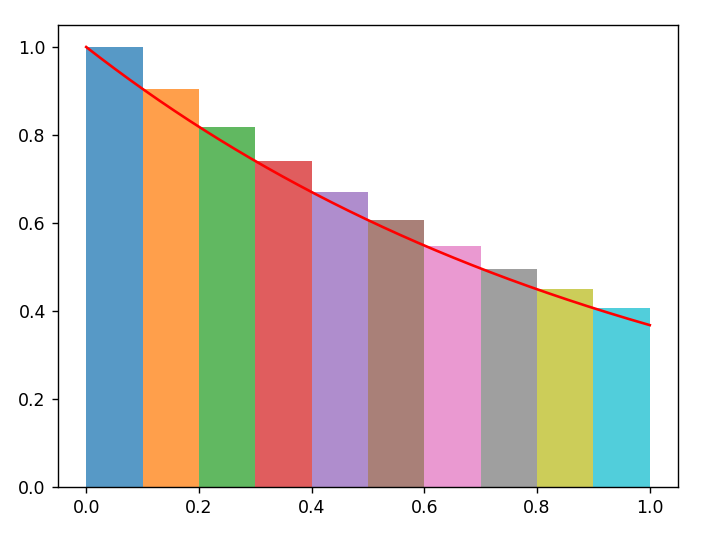
\includegraphics[width = 10cm, height = 7cm]{left_10.png}\\
	n = 10. Ранг разбиения 0.1. Результат: \(R \approx 0.66425\).\\
\end{frame}
\begin{frame}
	\large \textbf{\textcolor{structure.fg}{Метод левых прямоугольников}}\\[1cm]
	Формула погрешности:
	\[|R_n| \leq max_{x \in [a, b]} |f^\prime(x)| \frac{(b-a)^2}{2n}\]
	Тогда имеем:
	\[|R_n| \leq max_{x \in [0, 1]} |-e^{-x}| \frac{1}{2n} = \frac{1}{2n}\]
	Последнее равенство корректно в силу монотонности производной на отрезке [0, 1]\\
	При n = 10, \(|R_n| \leq 0.05\), \(|I - R|\approx 0.03213\). Т.е. погрешность рассчетов не превышает максимальную.
\end{frame}
\begin{frame}
	\large \textbf{\textcolor{structure.fg}{Метод правых прямоугольников}}\\
	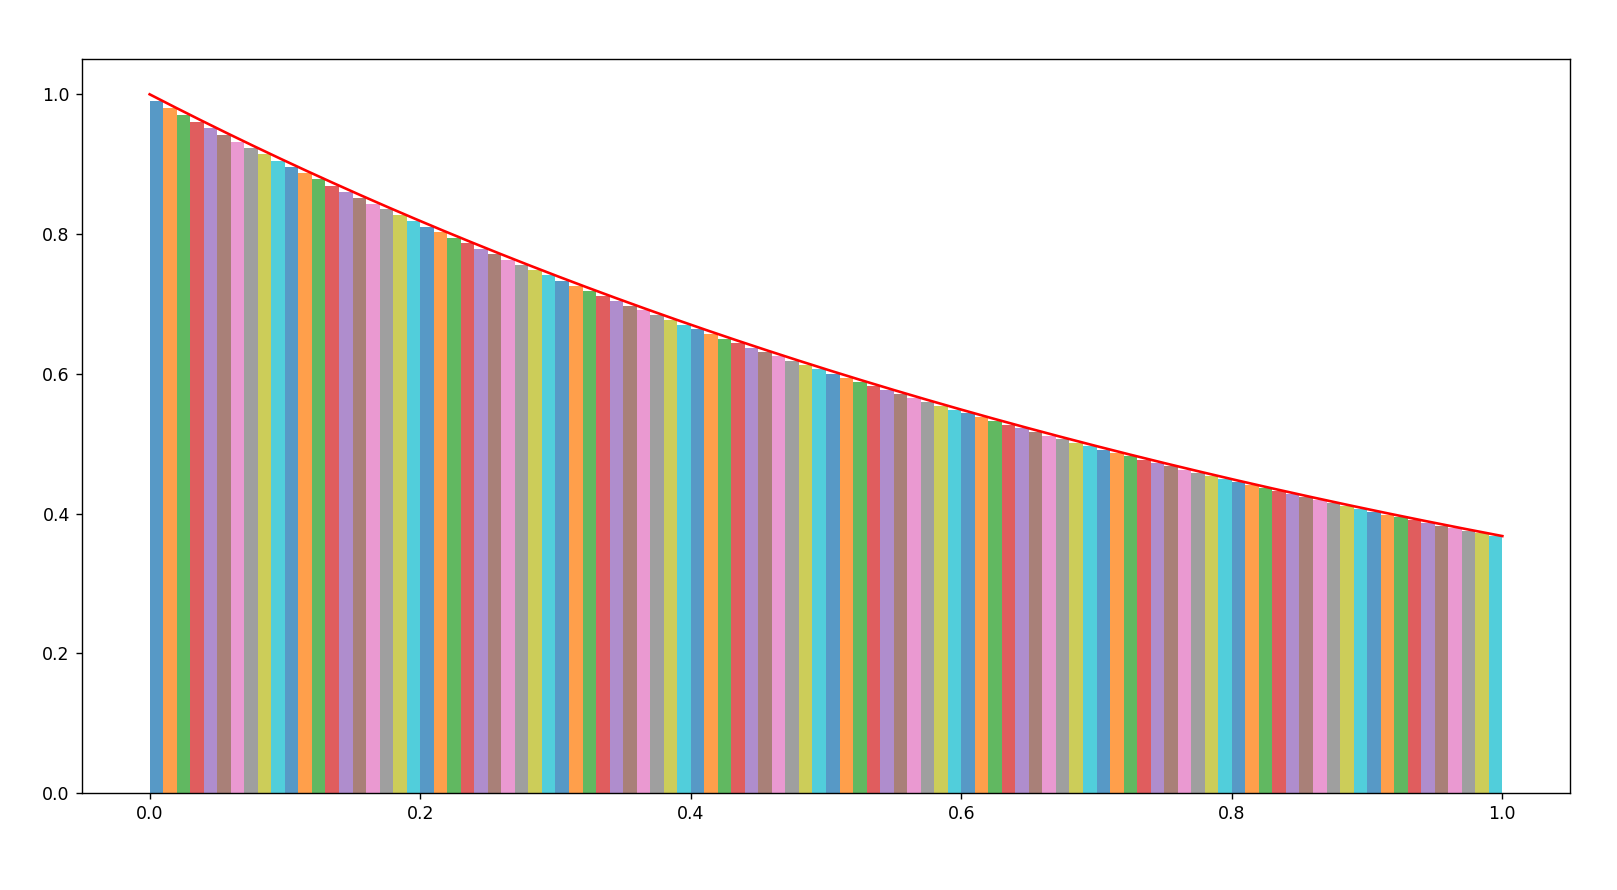
\includegraphics[width = 10cm, height = 6cm]{right_100.png}\\
	n = 100. Ранг разбиения 0.01. Результат: \(R \approx 0.62896\).
	Формула погрешности та же, что и в предыдущем методе:
	\[|R_n| \leq \frac{1}{2n}\]
	\end{frame}
	\begin{frame}
		\large \textbf{\textcolor{structure.fg}{Метод правых прямоугольников}}\\[1cm]
	При n = 100, \(|R_n| \leq 0.005\), \(|I - R|\approx 0.00316\). Т.е. погрешность рассчетов не превышает максимальную.
	\end{frame}
	\begin{frame}
		\large \textbf{\textcolor{structure.fg}{Метод трапеций}}\\
	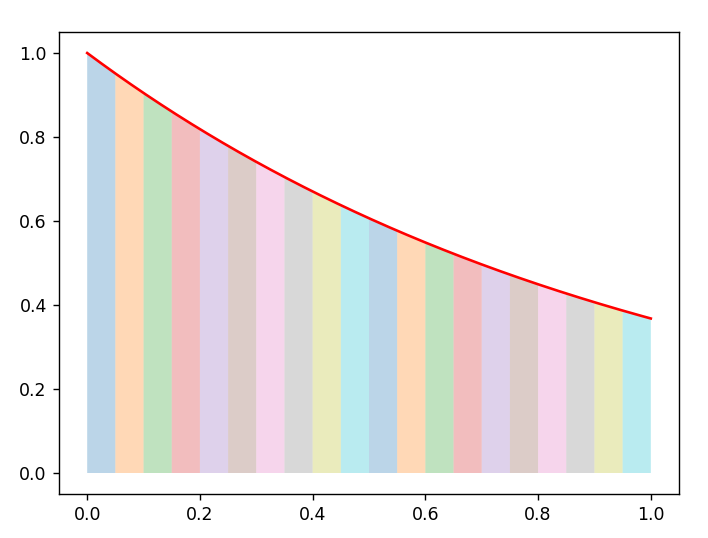
\includegraphics[width = 10cm, height = 7cm]{trap_10.png}\\
	n = 20. Ранг разбиения 0.05. Результат: \(R \approx 0.63225\).\\
\end{frame}
\begin{frame}
	\large \textbf{\textcolor{structure.fg}{Метод трапеций}}\\[1cm]
	Формула погрешности:
	\[|R_n| \leq max_{x \in [a, b]} |f^{\prime\prime}(x)| \frac{(b-a)^3}{12n^2}\]
	Тогда имеем:
	\[|R_n| \leq max_{x \in [0, 1]} |e^{-x}| \frac{1}{12n^2} = \frac{1}{12n^2}\]
	
	При n = 20, \(|R_n| \leq 0.00020...\), \(|I - R|\approx 0.00013\). Т.е. погрешность рассчетов не превышает максимальную.
	\end{frame}
	\begin{frame}
		\large \textbf{\textcolor{structure.fg}{Метод средних прямоугольников}}\\
	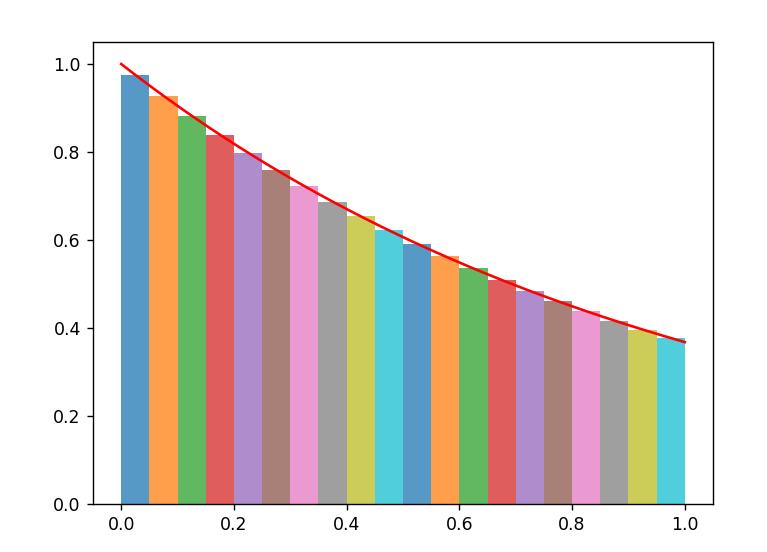
\includegraphics[width = 10cm, height = 7cm]{middle_200.png}\\
	n = 200. Ранг разбиения 0.005. Результат: \(R \approx 0.63211\).
\end{frame}
\begin{frame}
	\large \textbf{\textcolor{structure.fg}{Метод средних прямоугольников}}\\[1cm]
	Формула погрешности:
	\[|R_n| \leq max_{x \in [a, b]} |f^{\prime\prime}(x)| \frac{(b-a)^3}{24n^2}\]
	Тогда имеем:
	\[|R_n| \leq max_{x \in [0, 1]} |e^{-x}| \frac{1}{24n^2} = \frac{1}{24n^2}\]\\
	При n = 20, \(|R_n| \leq 0.00010...\), \(|I - R|\approx 0.00001\). Т.е. погрешность рассчетов не превышает максимальную.\\[1cm]
	
	Отметим, что \(e^{-x} \in C^2[0, 1]\), так что все 4 полученные оценки погрешности корректны. Для всех четырех методов выполняется: \(|R_n| \xrightarrow{n \to \infty}{} 0\).
	\end{frame}
	
	\large \textbf{\textcolor{structure.fg}{Индивидуальная часть. Ушаков Роман}}\\
	Дан интеграл:
	\[\int\limits_0^{\pi/2} \cos{2x} \, dx\]
	
	Для нахождения суммы для интеграла Римана на \([a, b]\) воспользуемся формулой правых прямоугольников:
	\[\lim\limits_{n\to\infty}\frac{b-a}{n}\sum^{n-1}_{i=0}{f(x^i)}\]
	
	В нашем случае:
	\[I=\lim\limits_{n\to\infty}\frac{\pi/2}{n}\sum^{n-1}_{k=0}{\cos{(2k \cdot \frac{\pi/2}{n})}}\]
	
	\vspace{0.2cm}
	
	
	\newpage
	
	2. \textbf{Вычисление суммы}
	
	Для вычисления суммы косинусов, воспользуемся данной формулой:
	\[\sum_{k=0}^{n-1} \cos(k \cdot \alpha) = \frac{\sin(n \alpha /2)}{\sin(\alpha / 2)} \cdot \cos(\frac{(n-1)\alpha}{2}), \text{ при } \sin(\alpha/2) \neq 0.\]
	
	Подставляем(\(\alpha = \frac{\pi}{n}\)):
	\[I=\lim\limits_{n\to\infty} (\frac{\pi/2}{n} \cdot \frac{\sin(\pi/2)}{\sin(\frac{\pi}{2n})} \cdot \sin(\frac{\pi}{2n}))=\lim\limits_{n\to\infty}\frac{\pi/2}{n}=0\]
	
	\vspace{0.2cm}
	\newpage
	3. \textbf{Проверка существования интеграла}
	
	Данная функция \(\cos(2x)\) непрерывна на отрезке \([a, b]\), что является достаточным условием для существования интеграла.
	
	\vspace{0.2cm}
	
	4. \textbf{Проверка прямым интегрированием}
	
	\[\int\limits_0^{\pi/2} \cos{2x} \, \left.dx=\frac{1}{2}\sin(2x)\right|_0^{\pi/2}=\frac{1}{2}\sin(\pi)-\frac{1}{2}\sin(0)=0.\]
	\newpage
	\large \textbf{\textcolor{structure.fg}{Часть 2. Численное интегрирование}}\\
	
	Задание выполнено на языке программирования Python.
	Для отрисовки графиков использовалась библиотека matplotlib.\\
	Значение исходного определенного интеграла: \(I=0\).\\
	Значение первой половины: \(I=0.5\)\\[1cm]
	\(\cos{2x} \in C^2[0, \pi/2]\), так что все следующие полученные оценки погрешности корректны. 
	
	\newpage
	
	\large \textbf{\textcolor{structure.fg}{Метод левых прямоугольников}}\\
	Вычисление ошибки: 
	\(|R_n|\leq \max\limits_{x\in[a,b]}{|f'(x)|\frac{(b-a)^2}{2n}}\) \\
	
	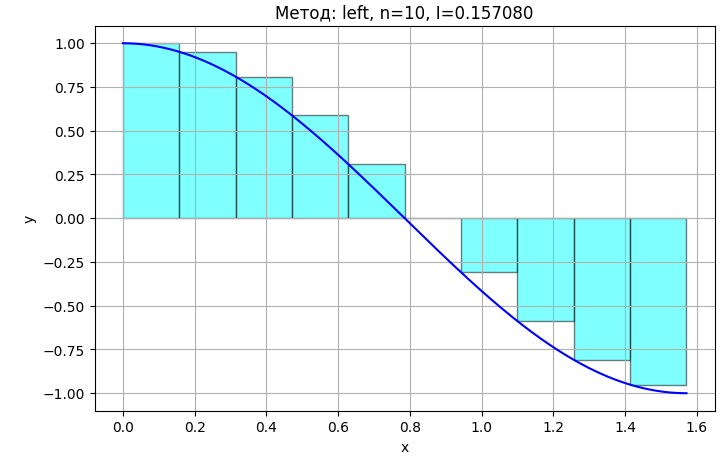
\includegraphics[width=0.6\linewidth]{left_n10.png}\\
	\(n=10, R = 0.157080\) \\
	\(|R_n|\leq \max\limits_{x\in[0,\pi/2]}{|-2\sin{2x}|\frac{(\pi/2)^2}{2n}}=
	2\ \cdot\ \frac{(\pi/2)^2}{2n}=\frac{\pi^2}{4n}\) \\
	\(|R_n|\leq \frac{\pi^2}{4n}=\frac{\pi^2}{4\cdot 10} \approx 0.246740\)\\
	\(|R_n| \leq 0.246740\), \(|R-I|\approx0.157080\),\\
	погрешность расчетов не превышает теоретическую.
	
	\vspace{0.5cm}
	
	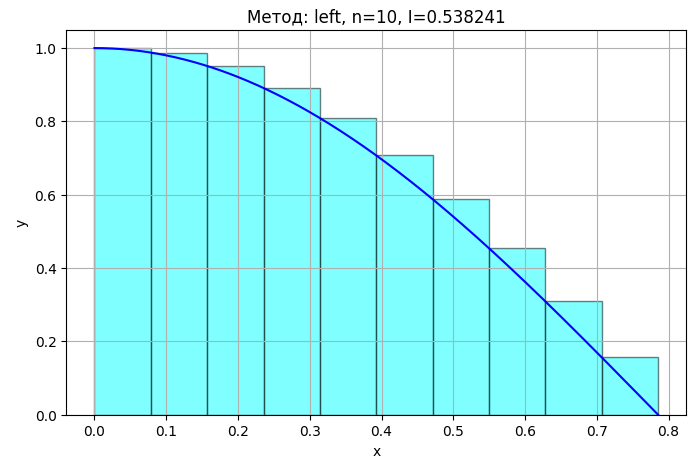
\includegraphics[width=0.6\linewidth]{left_half.png}\\
	\(n=10, R = 0.538241\) \\
	\(|R_n|\leq \max\limits_{x\in[0,\pi/4]}{|-2\sin{2x}|\frac{(\pi/4)^2}{2n}}=
	2\ \cdot\ \frac{(\pi/4)^2}{2n}=\frac{\pi^2}{16n}\) \\
	\(|R_n|\leq \frac{\pi^2}{16n}=\frac{\pi^2}{16\cdot 10} \approx 0.061685\)\\
	\(|R_n| \leq 0.061685\), \(|R-I|\approx0.038241\),\\
	погрешность расчетов не превышает теоретическую.
	
	
	\newpage
	
	\large \textbf{\textcolor{structure.fg}{Метод правых прямоугольников}}\\
	Вычисление ошибки: 
	\(|R_n|\leq \max\limits_{x\in[a,b]}{|f'(x)|\frac{(b-a)^2}{2n}}\)\\
	
	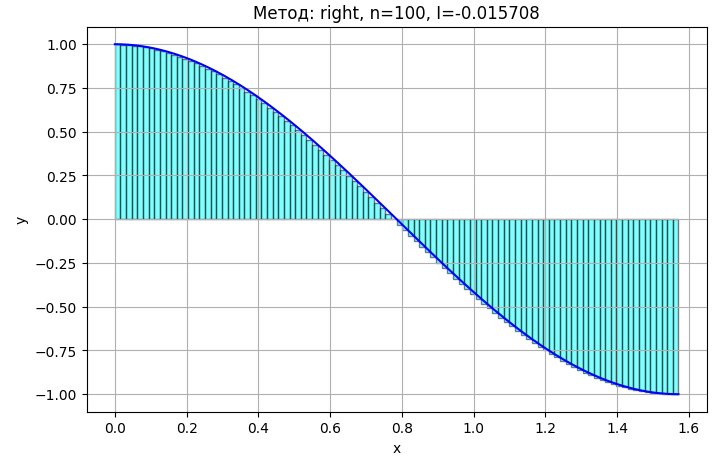
\includegraphics[width=0.6\linewidth]{right_n100.png}\\
	\(n=100, R=-0.015708\) \\
	\(|R_n|\leq \frac{\pi^2}{4n}=\frac{\pi^2}{4\cdot 100} \approx 0.024674\)\\
	\(|R_n| \leq 0.024674\), \(|R-I|\approx0.015708\),\\
	погрешность расчетов не превышает теоретическую.
	
	\vspace{0.5cm}
	
	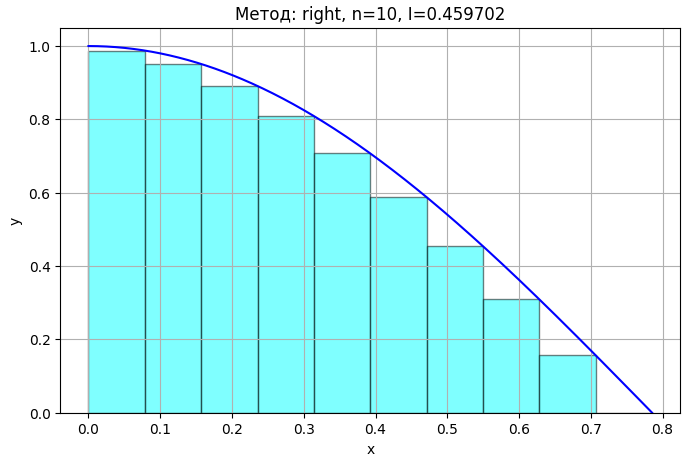
\includegraphics[width=0.6\linewidth]{right_half.png}\\
	\(n=10, R=0.459702\) \\
	\(|R_n|\leq \frac{\pi^2}{16n}=\frac{\pi^2}{16\cdot 10} \approx 0.061685\)\\
	\(|R_n| \leq 0.061685\), \(|R-I|\approx 0.040298\),\\
	погрешность расчетов не превышает теоретическую.
	
	
	\newpage
	
	\large \textbf{\textcolor{structure.fg}{Метод средних прямоугольников}}\\
	Вычисление ошибки:
	\(|R_n|\leq \max\limits_{x\in[a,b]}{|f''(x)|\frac{(b-a)^3}{24n^2}}\)\\
	
	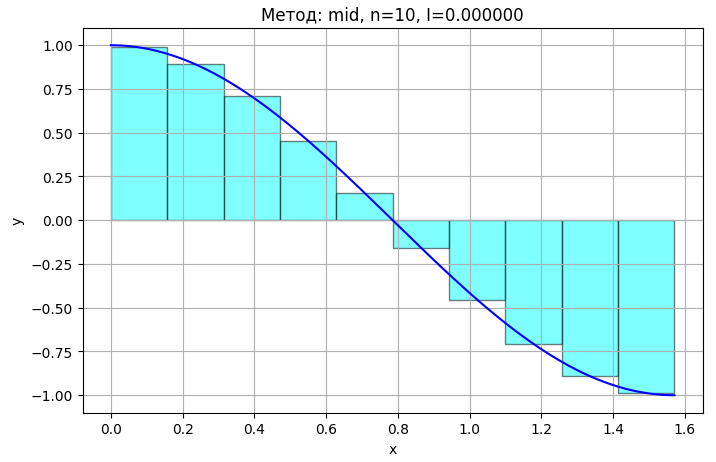
\includegraphics[width=0.6\linewidth]{mid_n10.png}\\
	\(n=10, R=0\) \\
	\(|R_n| \leq \max\limits_{x\in[0,\pi/2]}{|-4\cos{2x}|\frac{(\pi/2)^3}{24n^2}}=\frac{\pi^3}{48n^2}\)\\
	\(|R_n|\leq \frac{\pi^3}{48n^2}=\frac{\pi^3}{48\cdot 100} \approx 0.006459\)
	\(|R_n| \leq 0.006459\), \(|R-I| \approx 0\),\\
	погрешность расчетов не превышает теоретическую.
	
	\vspace{0.5cm}
	
	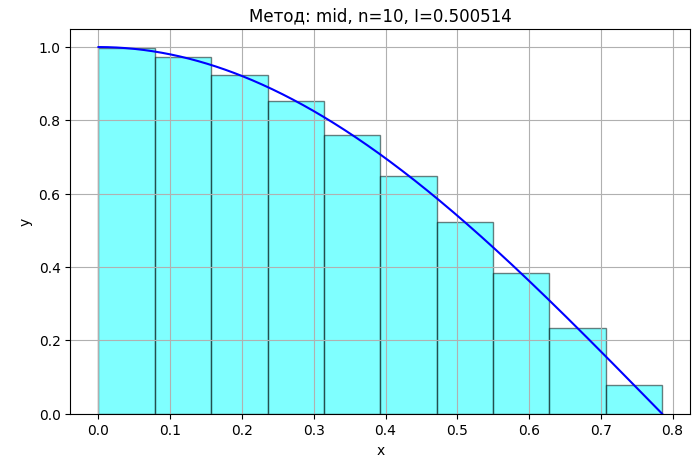
\includegraphics[width=0.6\linewidth]{mid_half.png}\\
	\(n=10, R=0.500514\) \\
	\(|R_n| \leq \max\limits_{x\in[0,\pi/2]}{|-4\cos{2x}|\frac{(\pi/4)^3}{24n^2}}=\frac{\pi^3}{384n^2}\)\\
	\(|R_n|\leq \frac{\pi^3}{384n^2}=\frac{\pi^3}{384\cdot 100} \approx 0.000807\)
	\(|R_n| \leq 0.000807\), \(|R-I| \approx 0.000514\),\\
	погрешность расчетов не превышает теоретическую.
	
	
	\newpage
	
	\large \textbf{\textcolor{structure.fg}{Метод трапеций}}\\
	Вычисление ошибки: 
	\(|R_n|\leq \max\limits_{x\in[a,b]}{|f''(x)|\frac{(b-a)^3}{12n^2}}\)\\
	
	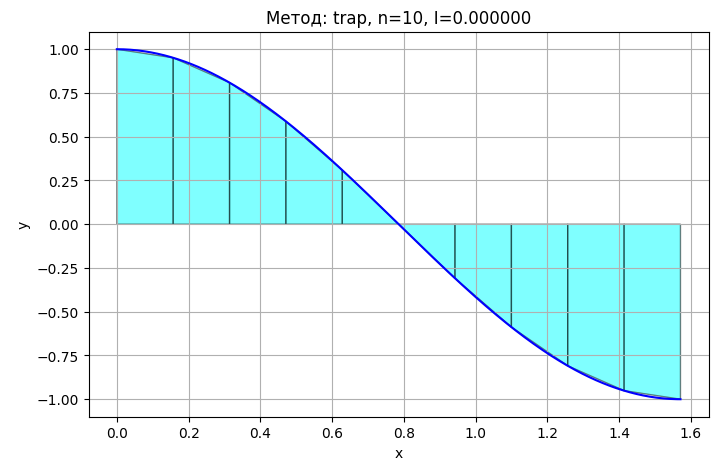
\includegraphics[width=0.7\linewidth]{trap_n10.png}\\
	\(n=10, R=0\) \\
	\(|R_n| \leq \frac{\pi^3}{24n^2}=\frac{\pi^3}{24\cdot 100} \approx 0.0129192\)
	\(|R_n| \leq 0.0129192\), \(|R-I| \approx 0\),\\
	погрешность расчетов не превышает теоретическую.
	
	\vspace{0.3cm}
	
	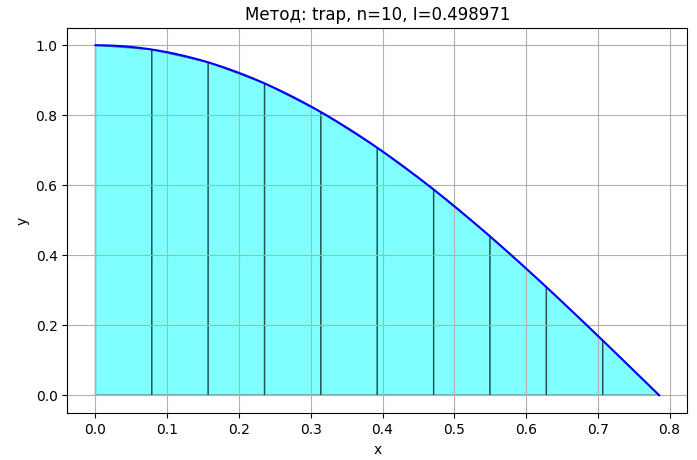
\includegraphics[width=0.7\linewidth]{trap_half.png}\\
	\(n=10, R=0.498971\) \\
	\(|R_n| \leq \frac{\pi^3}{192n^2}=\frac{\pi^3}{192\cdot 100} \approx 0.001614\)
	\(|R_n| \leq 0.001614\), \(|R-I| \approx 0.001029\),\\
	погрешность расчетов не превышает теоретическую.
	
	Отметим, что для всех четырех методов выполняется: \(|R_n| \xrightarrow{n \to \infty}{} 0\).
	\newpage
	\large \textbf{\textcolor{structure.fg}{Индивидуальная часть. Веселов Фёдор}}\\
	\[f(x) = sinx, [0, \pi]\]
	\[0 < x_1 < x_2 < ... < x_n < \pi\]
	\[\Delta x_i = x_i - x_{i-1}\]
	\[ \int_0^\pi f(x) \, dx \approx \sum_{i=1}^n f(\xi_i)\Delta x_i = 
	\sum_{i=1}^n sin(\xi_i)\Delta x_i \]
	\newpage
	Пусть, так как у нас разбиение равномерное:
	\[\forall i,j: 
	\Delta x_i = \Delta x_j \implies \Delta x_i = 
	\frac{\pi - 0}{n} = \frac{\pi}{n}\]
	\[\text{Пусть } \xi_i = x_i = i\cdot\frac{\pi}{n} = \frac{i\pi}{n}\]
	\[\implies \sum_{i=1}^n sin(\frac{i\pi}{n})\cdot \frac{\pi}{n}
	= \frac{\pi}{n}\sum_{i=1}^n sin(\frac{i\pi}{n})\]
	\newpage
	\textbf{Нахождение интегральной суммы}
	\[
	\lim_{n \to \infty} \frac{\pi}{n}\sum_{i=1}^n sin(\frac{i\pi}{n}) =
	\lim_{n \to \infty} \frac{\pi}{n}\sum_{i=1}^n \frac{sin(\frac{i\pi}{n})\cdot2sin(\frac{\pi}{n})}{2sin(\frac{\pi}{n})} \overset{(*)}{=}
	\]
	\[
	(*): sin(\frac{i\pi}{n})\cdot2sin(\frac{\pi}{n}) = 
	cos(\frac{i\pi}{n} - \frac{\pi}{2n}) - cos(\frac{i\pi}{n} + \frac{\pi}{2n})
	=\]\[ cos(\frac{\pi}{n}(i-\frac{1}{2})) - cos(\frac{\pi}{n}(i+\frac{1}{2}))
	\]
	\[
	\overset{(*)}{=} \lim_{n \to \infty} \frac{\pi}{n}\cdot\frac{1}{2sin(\frac{\pi}{2n})}\cdot
	\biggl(cos\Bigl(\frac{\pi}{n}\frac{1}{2}\Bigr) - \cancel{cos\Bigl(\frac{\pi}{n}\cdot\frac{3}{2}\Bigr)} + \cancel{cos\Bigl(\frac{\pi}{n}\cdot\frac{3}{2}\Bigr)}
	- \cancel{...} + \]\[\cancel{cos\Bigl(\frac{\pi}{n}\cdot\frac{2n-1}{2}\Bigr)} - cos\Bigl(\frac{\pi}{n}\cdot\frac{2n+1}{2}\Bigr)\biggr) =
	\]
	\newpage
	\[
	= \lim_{n \to \infty} \frac{\pi}{n}\Biggl( 
	\frac{cos\Bigl(\frac{\pi}{2n}\Bigr) - cos\Bigl(\pi+\frac{\pi}{2n}\Bigr)}{2sin(\frac{\pi}{2n})} \Biggr) =
	\lim_{n \to \infty} \frac{\pi}{n} \cdot 
	\frac{\cancel{2}cos(\frac{\pi}{2n})}{\cancel{2}sin(\frac{\pi}{2n})}
	=\]\[ = \lim_{n \to \infty} \underbrace{\frac{\frac{\pi}{2n}}{\sin(\frac{\pi}{2n})}}_{\to1} \cdot 
	\underbrace{2\cos\left(\frac{\pi}{2n}\right)}_{\to 2} = 2
	\]
	\newpage
	\textbf{Доказательство того, что интеграл существует}\\
	Функция f(x) = sin(x) непрерывна на отрезке  $[0,\pi]$ , а следовательно по критерию интегрируемости Римана она интегрируема $\implies $
	\[\exists \int_0^\pi f(x) \, dx =  \int_0^\pi sin(x) \, dx \]
	
	\textbf{Нахождение через определенный интеграл}
	\[
	\int_0^\pi f(x) \, dx = \int_0^\pi sin(x) \, dx = \Bigl[-cos(x)\Bigr]\Bigg|_0^\pi =\]\[
	-\Bigl[cos(\pi) - cos(0)\Bigr] = -\Bigl[-1 - 1\Bigr] = 2 
	\]
	Значения интеграла вычисленные разными способами совпадают.
	\newpage
	\large \textbf{\textcolor{structure.fg}{Графики интегральных сумм}}\\
	\textbf{Метод левых прямоугольников}
	
\includegraphics[width=0.5\textwidth]{Sin_left.png}
	\\n = 31; Ранг разбиения: 0.1; S\textsubscript{гр} = 1.9953899
	Формула погрешности для метода левых прямоугольников:
	$$|R_n| \le \max_{x \in [a, b]} |f'(x)| \frac{(b - a)^2}{2n}$$
	\newpage
	В нашем случае: 
	$$|R_n| \le \max_{x \in [0, \pi]} |-sin(x)| \frac{\pi^2}{2n} = \frac{\pi^2}{2n} $$
	$$ n = 31 \implies R_n \leq \frac{\pi^2}{62} < 0.15919$$ 
	$$ |S_\text{ист} - S_\text{гр}| = 0,0046101 < 0,15 < R_n \implies \text{Рассчитано корректно}$$
	\newpage
	\textbf{Метод правых прямоугольников}
	
\includegraphics[width=0.5\textwidth]{Sin_right.png}
	\\n = 13; Ранг разбиения: 0.24; S\textsubscript{гр} = 1.9927496961573818
	Формула погрешности для метода правых прямоугольников(такая же):
	$$|R_n| \le \max_{x \in [a, b]} |f'(x)| \frac{(b - a)^2}{2n}$$
	\newpage
	В нашем случае: 
	$$|R_n| \le \max_{x \in [0, \pi]} |cos(x)| \frac{\pi^2}{2n} = \frac{\pi^2}{2n} $$
	$$ n = 13 \implies R_n \leq \frac{\pi^2}{26} < 0.37960017$$ 
	$$ |S_\text{ист} - S_\text{гр}| = 0.007250304 < 0.008 < R_n \implies \text{Рассчитано корректно}$$
	\newpage
	\textbf{Метод средних прямоугольников}
	
\includegraphics[width=0.5\textwidth]{Sin_middle.png}
	\\n = 18; Ранг разбиения: 0.17; S\textsubscript{гр} = 1.9990795211790413
	Формула погрешности для метода средних прямоугольников:
	$$|R_n| \le \max_{x \in [a, b]} |f''(x)| \frac{(b - a)^3}{24n^2}$$
	\newpage
	В нашем случае: 
	$$|R_n| \le \max_{x \in [0, \pi]} |cos(x)| \frac{\pi^3}{24n^2} = \frac{\pi^3}{24n^2} $$
	$$ n = 18 \implies R_n \leq \frac{\pi^3}{7776} < 0,003987432700656 $$ 
	$$ |S_\text{ист} - S_\text{гр}| = 0.0009204788209587 < R_n \implies \text{Рассчитано корректно}$$
	\newpage
	\textbf{Метод трапеций}
	
\includegraphics[width=0.5\textwidth]{Sin_trap.png}
	\\n = 34; Ранг разбиения: 0.9; S\textsubscript{гр} = 1.9953252293472543
	Формула погрешности для метода трапеций:
	$$|R_n| \le \max_{x \in [a, b]} |f''(x)| \frac{(b - a)^3}{12n^2}$$
	\newpage
	В нашем случае: 
	$$|R_n| \le \max_{x \in [0, \pi]} |-cos(x)| \frac{(\pi - 0)^3}{12n^2} = \frac{\pi^3}{12n^2} $$
	$$ n = 34 \implies R_n \leq \frac{\pi^3}{13872} < 0,0032351 $$ 
	$$ |S_\text{ист} - S_\text{гр}| = 0.003174771 < R_n \implies \text{Рассчитано корректно}$$
	
	
	\newpage
	\textbf{Нахождение погрешности оценки}
	\[
	\Delta = \Bigg| \int_0^\pi f(x) \, dx - S_n \Bigg| = \Bigg| 2 - \frac{\pi}{n}ctg\Bigl(\frac{\pi}{2n}\Bigr) \Bigg|
	\]
	
	Теориетиеская погрешность:  \[|R_n| \leq \max_{x \in [0,\pi]}|f'(x)|\frac{(\pi-0)^2}{2n}
	= \max_{x \in [0,\pi]}\Bigl[\frac{\pi^2}{2n}cos(x)\Bigr] = \frac{\pi^2}{2n}  
	\]
	Использем разложение котангенса в ряд Лорана в окрестности нуля:
	\[ \cot(t) = \frac{1}{t} - \frac{t}{3} - \frac{t^3}{45} + O(t^5) \]
	\newpage
	Подставим $t = \frac{h}{2}(h=\pi x=\frac{\pi}{n})$:
	\[ \Delta(h) = \left| 2 - h \left( \frac{1}{h/2} - \frac{h/2}{3} + O(h^3) \right) \right| \]
	\[ \Delta(h) = \left| 2 - \left( 2 - \frac{h^2}{6} + O(h^4) \right) \right| \]
	\[ \Delta(h) = \frac{h^2}{6} + O(h^4) \implies
	R_n \sim O(\frac{1}{n})\]
	\[\Delta \sim O(\frac{1}{n^2})\]
	\newpage
	\bigskip
	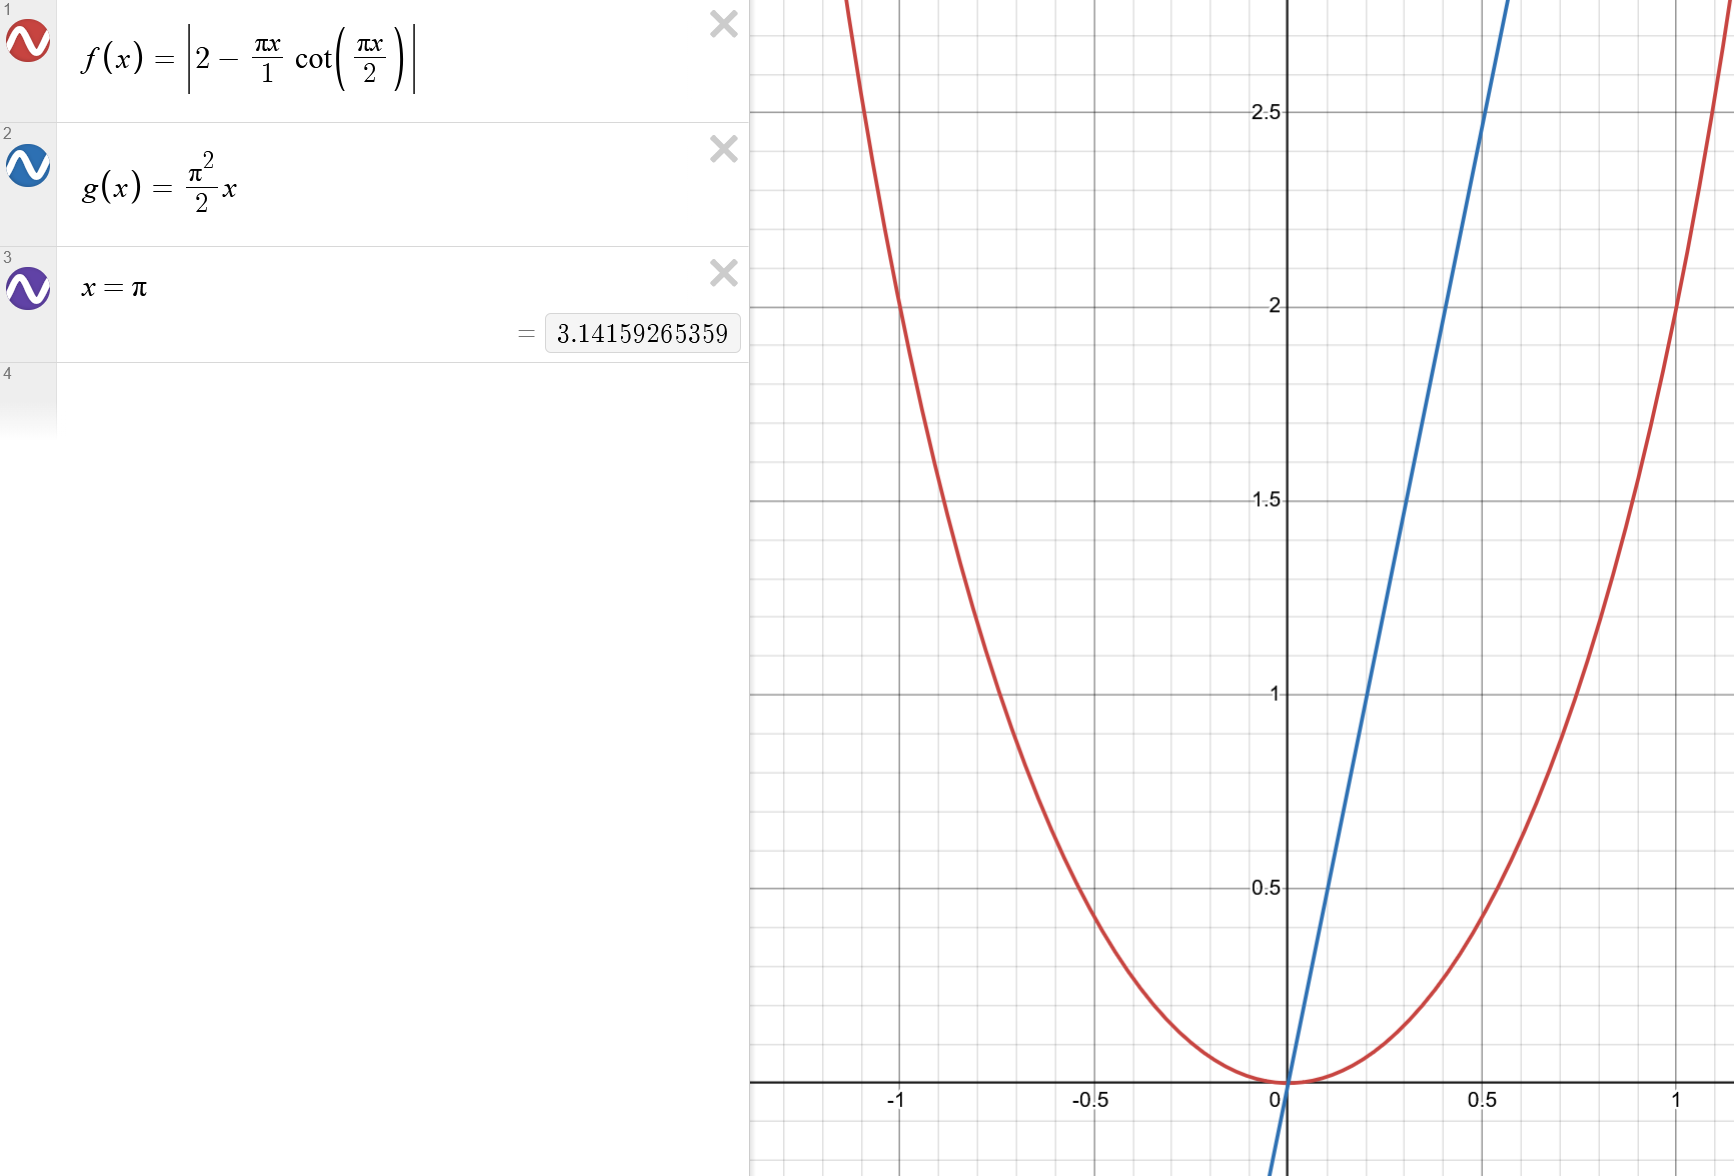
\includegraphics[width = 9cm, height = 7cm]{Погрешности.png}
	
	\[\text{Графики погрешностей при } n\to\infty \text{ }(x\to0)\] 
	
	\newpage
	\large \textbf{\textcolor{structure.fg}{Индивидуальная часть. Босенко Борис}}\\
	
		\large \textbf{\textcolor{structure.fg}{Аналитическая часть}}\\
	Дана функция:  $f(x) = x^2$\\
	Тогда предел интегральных сумм Римана будет выглядеть как 
	\[I = \lim_{\Delta x \to 0} \sum_{k=1}^{n} f(\xi_k)\Delta x \]
	
	Так как разбиение равномерное, для числа разбиений n можем посчитать координаты точек разбиения по формуле
	
	\[x_k = 1 + \frac{k}{n} ( 2 - 1 ) = 1 + \frac{k}{n}, k \in \{0, ..., n\}\]
	\newpage
	Тогда можем посчитать данный интеграл с помощью \textcolor{orange}{формулы правых прямоугольников:}
	
	\[ I = \lim_{\Delta x \to 0} \sum_{k=1}^{n} f(\xi_k)\Delta x = \lim_{\frac{1}{n} \to 0} \sum_{k=1}^{n} \left( f\left(1 + \frac{k}{n}\right) \frac{1}{n} \right) =\]\[ \lim_{n \to \infty} \left( \frac{1}{n} \sum_{k=1}^{n} \left( 1 + \frac{k}{n}\right)^2 \right)  = \lim_{n \to \infty} \left( \frac{1}{n} \sum_{k=1}^{n} \left( 1 + 2\frac{k}{n} + \frac{k^2}{n^2} \right)  \right)  = \]\[ = \lim_{n \to \infty} \left( \frac{1}{n} \left( n + \frac{n(n+1)}{n} + \frac{n(n+1)(2n+1)}{6n^2} \right)  \right)  = \] 
	\[ = \lim_{n \to \infty} \left( 1 + \frac{n+1}{n} + \frac{(n+1)(2n+1)}{6n^2} \right)  = \]\[1 + \lim_{n \to \infty} \frac{n+1}{n} + \lim_{n \to \infty} \frac{2n^2 + 3n + 1}{6n^2} = 1 + 1 + \frac{1}{3} = 2\frac{1}{3} = \frac{7}{3}\]
	\newpage
	При этом функция $f(x) = x^2$ интегрируема на промежутке $[1, 2]$, так как она непрерывна (и это является достаточным условием для существования интеграла.)
	
	Для сравнения, \textcolor{orange}{найдем значение этого интеграла по формуле Ньютона-Лейбница}:
	
	\[ \int_{1}^{2} f(x) dx = \int_{1}^{2} x^2 dx = \frac{x^3}{3} \ \bigg|_{1}^{2} = \frac{8}{3} - \frac{1}{3} = \frac{7}{3}\]
	
	Таким образом, \textcolor{orange}{оба способа дали одинаковый результат}.
	
	\newpage
	
	\addcontentsline{toc}{chapter}{Результаты работы программы}
	\section*{Результаты работы программы}
	
	\begin{center}
		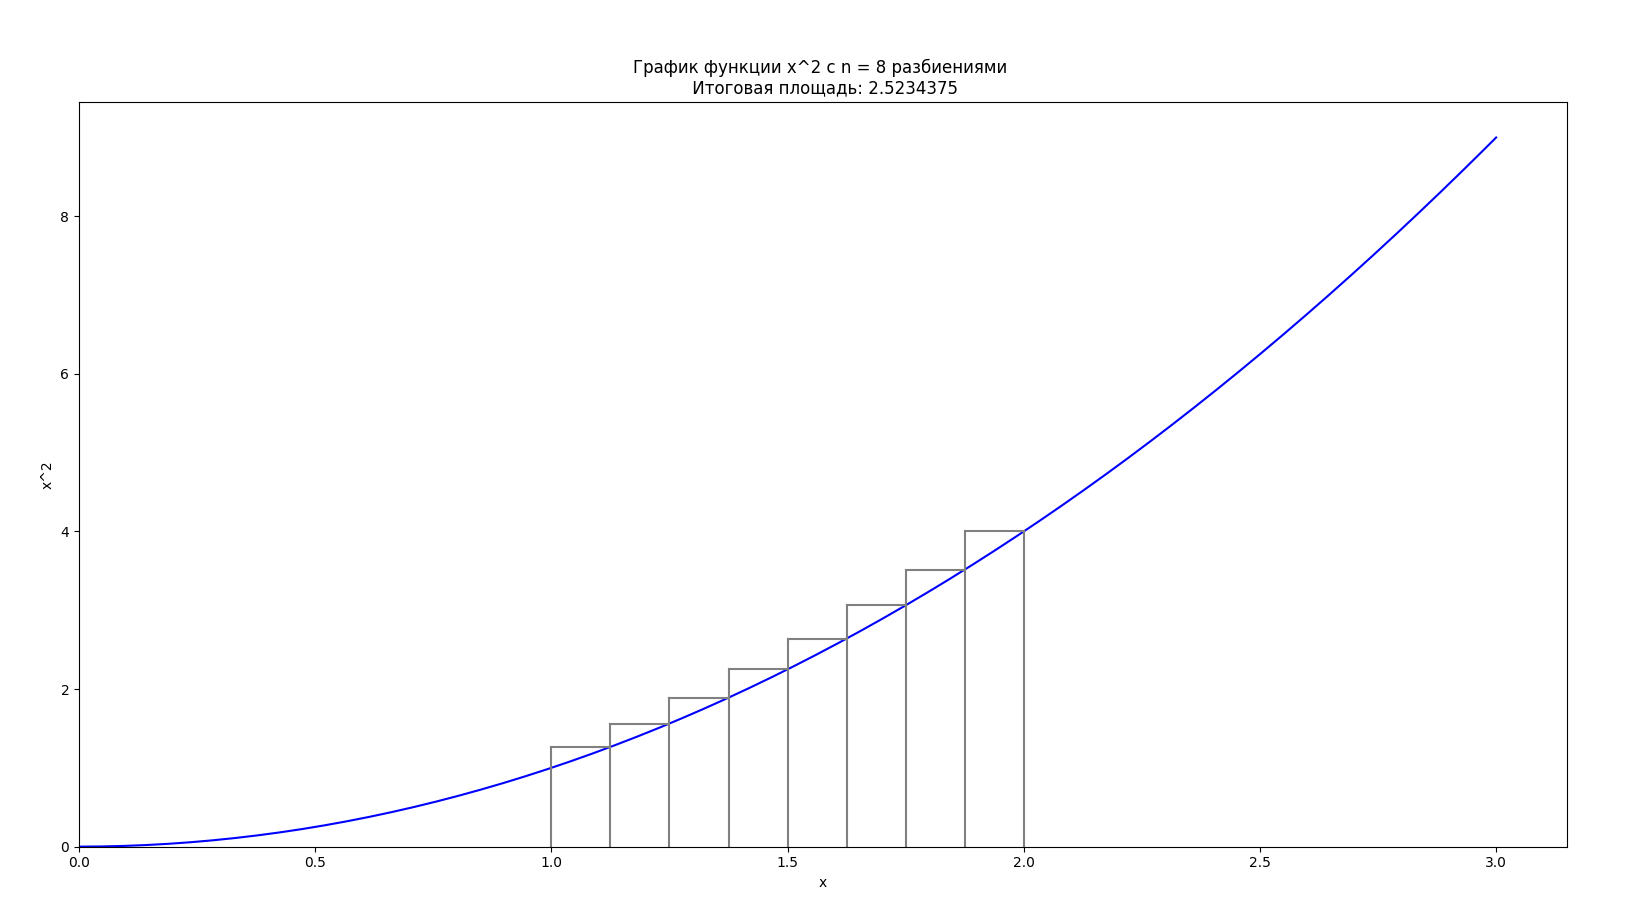
\includegraphics[width=9cm, height = 7cm]{Правые прямоугольники.png}
		Рисунок 1
		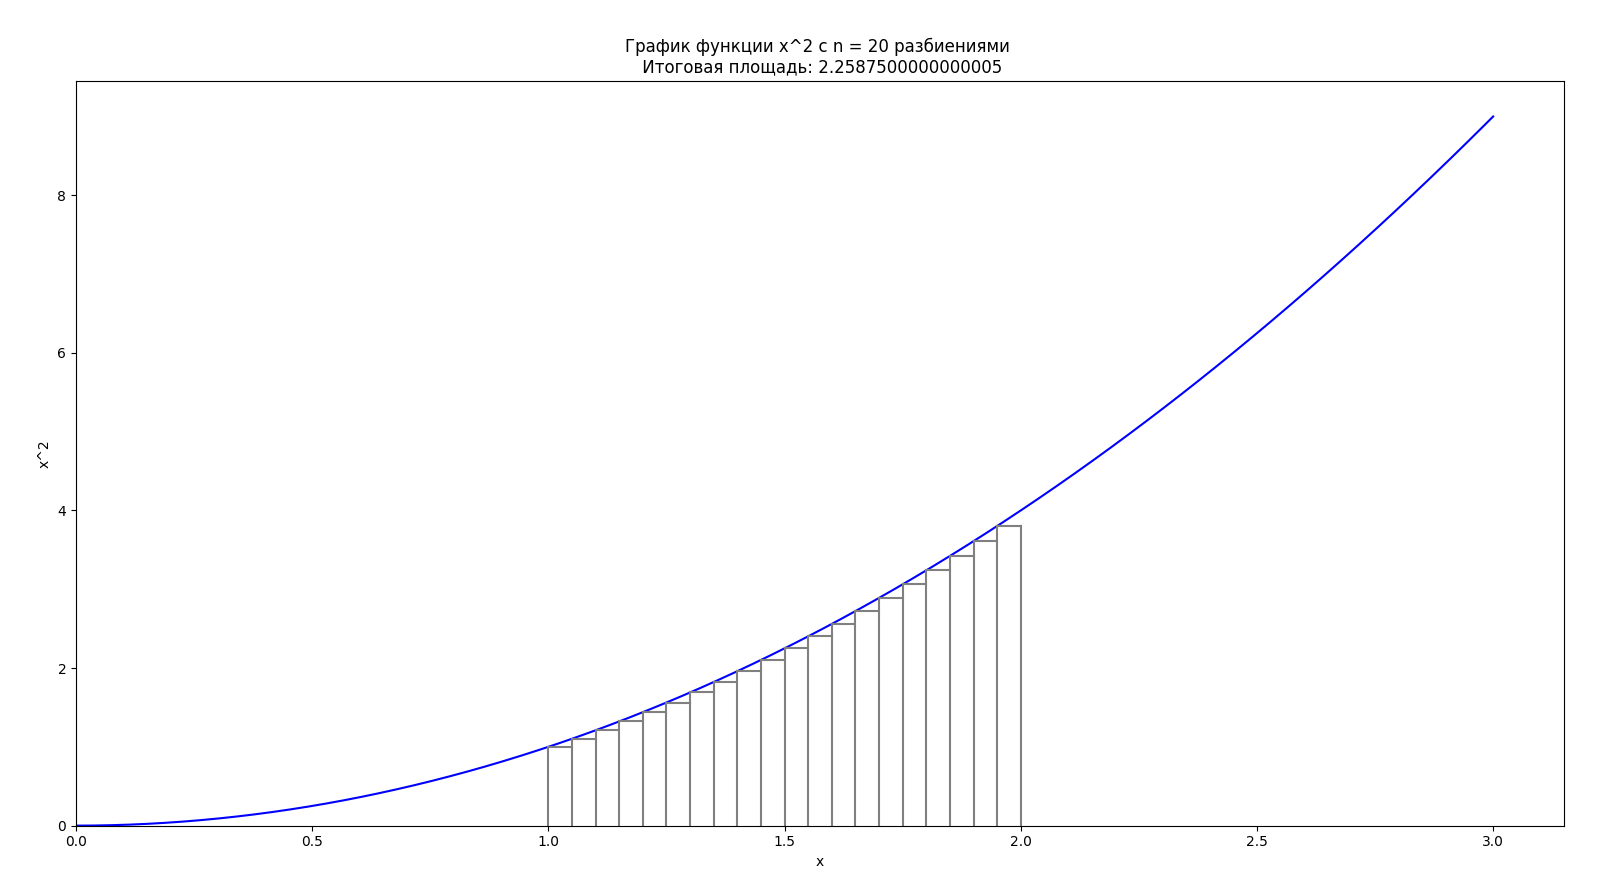
\includegraphics[width=9cm, height = 7cm]{Левые прямоугольники.png}
		Рисунок 2
		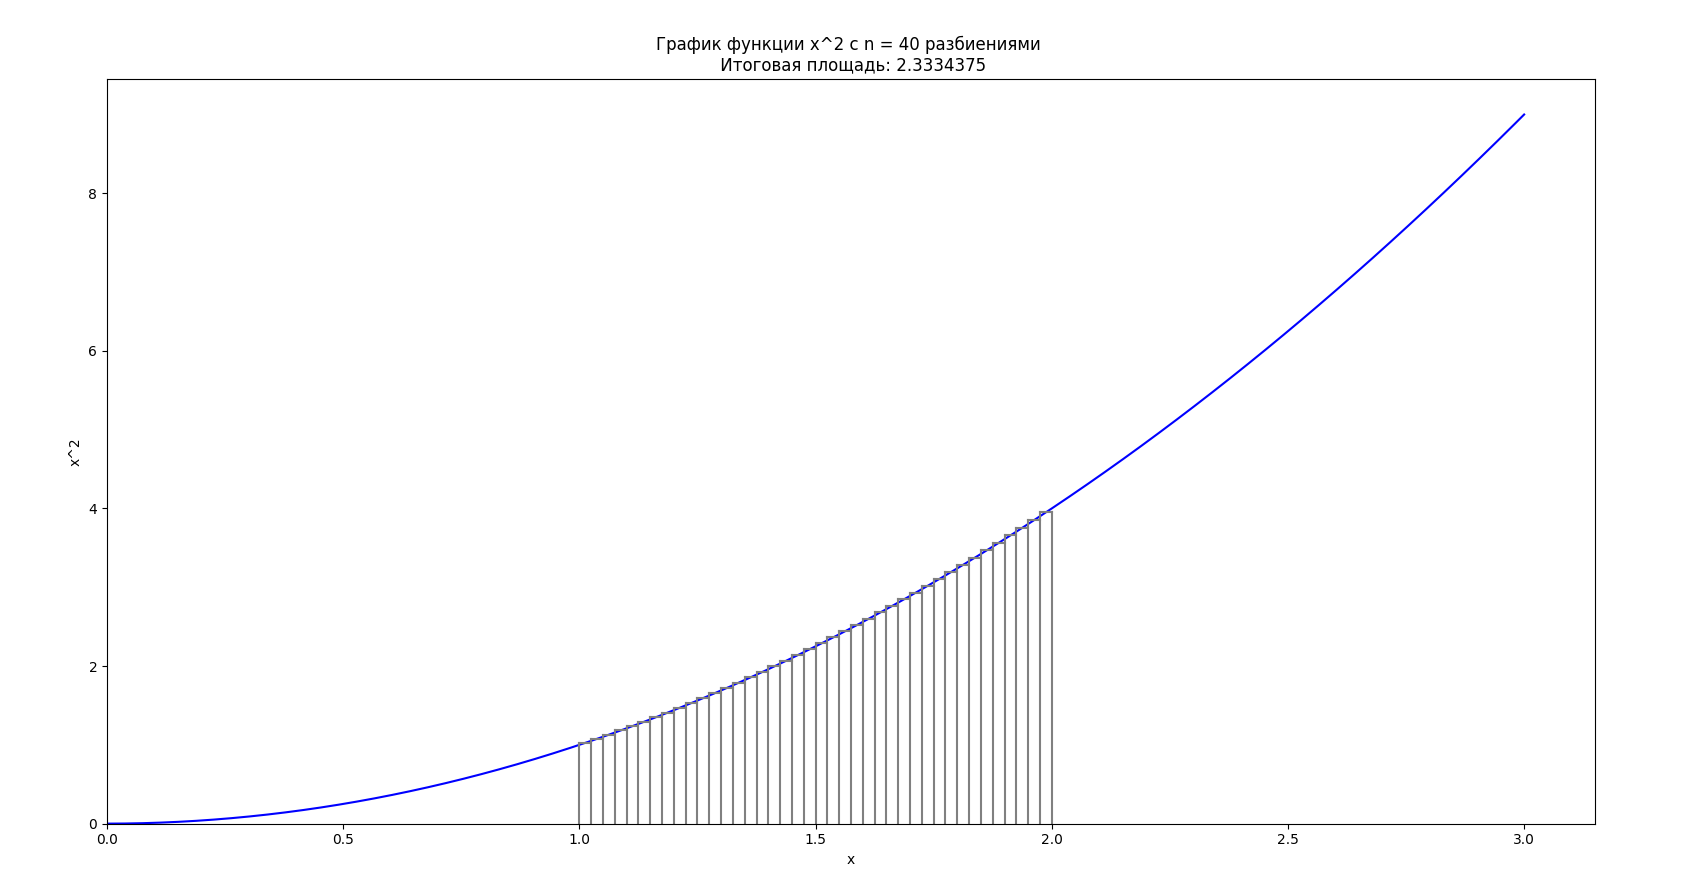
\includegraphics[width=9cm, height = 7cm]{Средние прямоугольники.png}
		Рисунок 3
		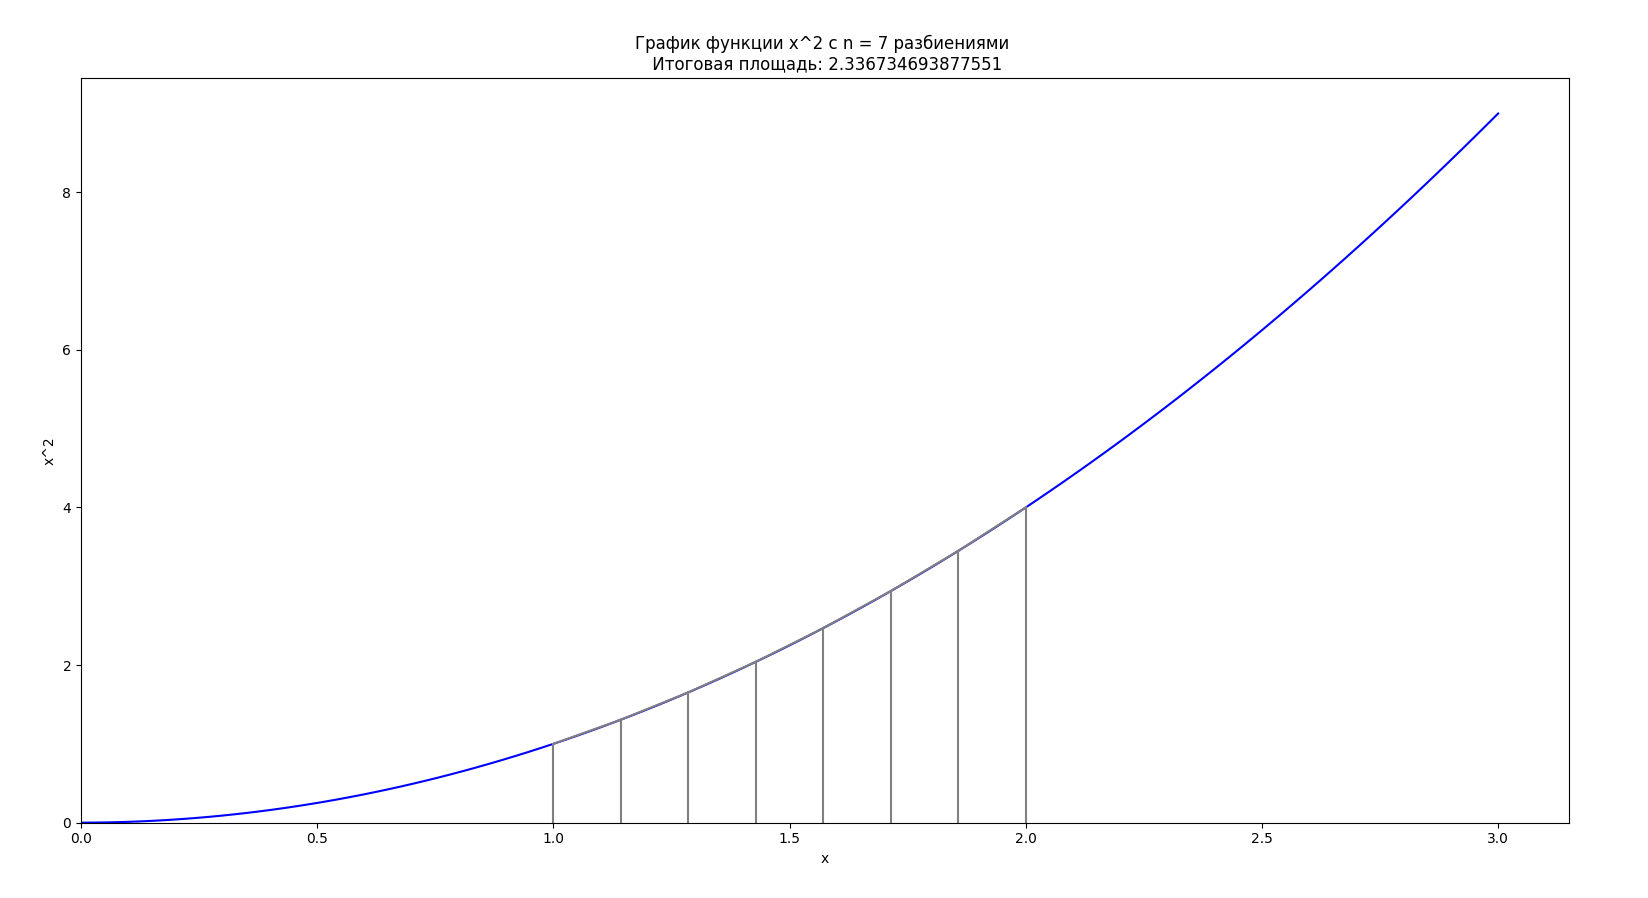
\includegraphics[width=9cm, height = 7cm]{Трапеции.png}
		Рисунок 4
	\end{center}
	
	\newpage
	
	\large \textbf{\textcolor{structure.fg}{Вывод формул для погрешностей}}\\
	\section*{Вывод формул для погрешностей}
	
	\textbf{Формула левых прямоугольников}
	
	Пусть $f \in C^1[a,b]$ \\ 
	Докажем формулу погрешности для левых прямоугольников. Для этого разложим функцию в ряд Тейлора с остатком в форме Лагранжа на промежутке $[x_{i-1}, x_i]$
	
	\[ f(x) = f(x_{i-1}) + f'(\xi)(x - x_{i-1}), \ \xi \in (x_{i-1}, x)\]
	
	Далее проинтегрируем обе части по отрезку $[x_{i-1}, x_i]$
	
	\[ \int\limits_{x{i-1}}^{x_i} f(x)dx = \int\limits_{x_{i-1}}^{x_i} f(x_{i-1})dx + \int\limits_{x_{i-1}}^{x_i} f'(\xi)(x - x_{i-1})dx\]
	\newpage
	Первый интеграл в правой части можно заменить на $f(x_{i-1}) \Delta x_i$, так как он равен площади одного прямоугольника, а значит выражение принимает вид:
	
	\[ \int\limits_{x{i-1}}^{x_i} f(x)dx = f(x_{i-1}) \Delta x_i + \int\limits_{x_{i-1}}^{x_i} f'(\xi)(x - x_{i-1})dx\]
	
	Далее перенесем это слагаемое влево и используем оценку $f'(\xi) \leq \max_{\Delta_i} |f'(x)|$, таким образом получив
	
	\[ \left| \int\limits_{x{i-1}}^{x_i} f(x)dx - f(x_{i-1}) \Delta x_i \right| \leq \max_{\Delta_i} |f'(x)| \int\limits_{x_{i-1}}^{x_i} (x - x_{i-1})dx\]
	\newpage
	Упростим левое выражение, избавившись от интеграла
	\[ \max_{\Delta_i} |f'(x)| \int\limits_{x_{i-1}}^{x_i} (x - x_{i-1})dx = \max_{\Delta_i} |f'(x)| \int\limits_{x_{i-1}}^{x_i} (x - x_{i-1})d(x - x_{i-1}) = \]
	\[ = \max_{\Delta_i} |f'(x)| \frac{(x-x_{i-1})^2}{2} \Bigg|_{x_{i-1}}^{x_i} = \frac{1}{2} \max_{\Delta_i} |f'(x)| (x_i - x_{i-1})^2 \]
	\newpage
	Если $ \Delta x_i = \frac{b-a}{n}$, то, просуммировав по всем n отрезкам, получим:\\[1cm]
	\[ \left| \int\limits_{a}^{b} f(x)dx - \sum_{i=1}^{n} f(x_{i-1}) \Delta x_i \right| \leq \frac{(b-a)^2}{2n^2} \sum_{i=1}^{n} \max_{\Delta_i}|f'(x)|\leq\]\[ \leq \frac{(b-a)^2}{2n} \max_{[a, b]}|f'(x)|\]
	
	Таким образом, формула доказана.
	
	\newpage
	
	\textbf{Формула правых прямоугольников}
	
	Практически аналогично доказывается формула правых прямоугольников.
	
	Пусть $f \in C^1[a,b]$ \\ 
	Разложим функцию в ряд Тейлора с остатком в форме Лагранжа на промежутке $[x_{i-1}, x_i]$
	
	\[ f(x) = f(x_i) + f'(\xi)(x - x_i), \ \xi \in (x, x_i)\]
	
	Далее проинтегрируем обе части по отрезку $[x_{i-1}, x_i]$
	
	\[ \int\limits_{x{i-1}}^{x_i} f(x)dx = \int\limits_{x_{i-1}}^{x_i} f(x_i)dx + \int\limits_{x_{i-1}}^{x_i} f'(\xi)(x - x_i)dx\]
	
	Первый интеграл в правой части можно заменить на $f(x_i) \Delta x_i$, так как он равен площади одного прямоугольника, а значит выражение принимает вид 
	
	\[ \int\limits_{x{i-1}}^{x_i} f(x)dx = f(x_i) \Delta x_i + \int\limits_{x_{i-1}}^{x_i} f'(\xi)(x - x_i)dx\]
	
	Далее перенесем это слагаемое влево и используем оценку $f'(\xi) \leq \max_{\Delta_i} |f'(x)|$, таким образом получив
	
	\[ \left| \int\limits_{x{i-1}}^{x_i} f(x)dx - f(x_i) \Delta x_i \right| \leq \max_{\Delta_i} |f'(x)| \int\limits_{x_{i-1}}^{x_i} (x - x_i)dx\]
	\newpage
	Упростим левое выражение, избавившись от интеграла\\[1cm]

	\[ \max_{\Delta_i} |f'(x)| \int\limits_{x_{i-1}}^{x_i} (x - x_i)dx = \max_{\Delta_i} |f'(x)| \int\limits_{x_{i-1}}^{x_i} (x - x_i)d(x - x_i) = \]
	\[ = \max_{\Delta_i} |f'(x)| \frac{(x-x_i)^2}{2} \Bigg|_{x_{i-1}}^{x_i} = \frac{1}{2} \max_{\Delta_i} |f'(x)| (x_i - x_{i-1})^2 \]
	\newpage
	Если $ \Delta x_i = \frac{b-a}{n}$, то, просуммировав по всем n отрезкам, получим
	
	\[ \left| \int\limits_{a}^{b} f(x)dx - \sum_{i=1}^{n} f(x_i) \Delta x_i \right| \leq \frac{(b-a)^2}{2n^2} \sum_{i=1}^{n} \max_{\Delta_i}|f'(x)| \leq\]\[\leq \frac{(b-a)^2}{2n} \max_{[a, b]}|f'(x)|\]
	
	Таким образом, формула доказана.
	
	\newpage
	
	\textbf{Формула средних прямоугольников}
	
	Пусть $f \in C^2[a, b]$
	Введем $\overline{x} = \frac{x_{i-1} + x_i}{2}$ - средняя точка отрезка $[x_{i-1}, x_i]$. Разложим $f(x)$ в окрестности этой точки до второго порядка, и получим
	
	\[ f(x) = f(\overline{x}) + f'(\overline{x})(x - \overline{x}) + \frac{f''(\xi)}{2} (x - \overline{x})^2 dx, \ \xi \in [x, \overline{x}]\]
	
	Проинтегрируем обе части равенства по $[x_{i-1}, x_i]$
	
	\[ \int\limits_{x_{i-1}}^{x_i} f(x)dx = \int\limits_{x_{i-1}}^{x_i} f(\overline{x})dx + \int\limits_{x_{i-1}}^{x_i} f'(\overline{x})(x - \overline{x})dx + \int\limits_{x_{i-1}}^{x_i} \frac{f''(\xi)}{2} (x - \overline{x})^2 dx\]
	\newpage
	Упростим два первых слагаемых правой части. Для первого
	
	\[ \int\limits_{x_{i-1}}^{x_i} f(\overline{x})dx = f(\overline{x}) \Delta x\]
	
	так как этот интеграл - площадь среднего прямоугольника. Для второго слагаемого
	
	\[ \int\limits_{x_{i-1}}^{x_i} f'(\overline{x})(x - \overline{x})dx = f'(\overline{x})  \int\limits_{x_{i-1}}^{x_i} (x - \overline{x})d(x - \overline{x}) = f'(\overline{x}) \frac{(x - \overline{x})^2}{2} \Bigg|_{x_{i-1}}^{x_i} = 0 \]
	\newpage
	Тогда изначальное уравнение будет иметь вид 
	
	\[ \int\limits_{x_{i-1}}^{x_i} f(x)dx =  f(\overline{x}) \Delta x + \int\limits_{x_{i-1}}^{x_i} \frac{f''(\xi)}{2} (x - \overline{x})^2 dx\]
	
	или
	
	\[ \int\limits_{x_{i-1}}^{x_i} f(x)dx - f(\overline{x}) \Delta x = \int\limits_{x_{i-1}}^{x_i} \frac{f''(\xi)}{2} (x - \overline{x})^2 dx\]
	
	Далее воспользуемся оценкой $f''(\xi) \leq \max|f''(x)|$ и получим неравенство
	
	\[ \int\limits_{x_{i-1}}^{x_i} f(x)dx - f(\overline{x}) \Delta x \leq \frac{\max|f''(x)|}{2} \int\limits_{x_{i-1}}^{x_i} (x - \overline{x})^2 dx\]
	\newpage
	Упростим правую часть
	
	\[ \frac{\max|f''(x)|}{2} \int\limits_{x_{i-1}}^{x_i} (x - \overline{x})^2 d(x - \overline{x}) = \]\[\frac{\max|f''(x)|}{2} \frac{(x - \overline{x})^3}{3} \Bigg|_{x_{i-1}}^{x_i} = \frac{\max|f''(x)|(x_i - x_{i-1})^3}{24}\]
	
	Тогда получим неравенство
	
	\[ \int\limits_{x_{i-1}}^{x_i} f(x)dx - f(\overline{x}) \Delta x\ \leq \frac{\max|f''(x)|(x_i - x_{i-1})^3}{24}\]
	\newpage
	При $\Delta x = \frac{b-a}{n}$ просуммируем по всем отрезкам n и получим
	
	\[ \int\limits_{a}^{b} f(x)dx - \sum_{i=1}^{n} f(\overline{x}) \Delta x \leq \frac{\max|f''(x)|(\Delta x)^3}{24} = \]\[\max_{[a, b]}|f''(x)| \frac{(b - a)^3}{24n^2} \]
	
	Таким образом, формула доказана. \\
	\newpage
	\textbf{Формула трапеций}
	
	Пусть $f \in C^2[a, b]$
	
	Для каждого отрезка $[x_{i-1}, x_i]$ найдем значение функции $f(x)$ через линейный интерполяционный многочлен, тогда с учетом погрешности получим
	
	\[ f(x) = f(x_{i+1}) + \frac{f(x_i) - f(x_{i-1})}{\Delta x} (x - x_{i-1}) + \frac{f''(\xi)}{2}(x - x_{i-1})(x-x_i), \]\[ \xi \in [x_{i-1}, x_i]\]
	
	Проинтегрируем данное равенство. Таким образом для каждого отрезка получим погрешность
	
	\[ r_i  = \int\limits_{x_{i-1}}^{x_i} \frac{f''(\xi)}{2}(x - x_{i-1})(x-x_i)dx\]
	\newpage
	Применив оценку $f''(\xi) \leq \max|f''(x)|$, получим
	
	\[ r_i \leq \frac{\max|f''(x)|}{2} \left| \int\limits_{x_{i-1}}^{x_i}(x - x_{i-1})(x-x_i)dx \right| \]
	
	Посчитаем оставшийся интеграл. Для этого сделаем замену $t = x - x_{i-1}$, тогда $x - x_i = t - \Delta x, dx = dt, t_1 = 0, t_2 = \Delta x$. Получим
	
	\[ \int\limits_{0}^{\Delta x} t(t-\Delta x) dt = \int\limits_{0}^{\Delta x} t^2-t\Delta x dt = \left( \frac{t^3}{3} - \frac{t^2 \Delta x}{2} \right) \Bigg|_{0}^{\Delta x} = - \frac{(\Delta x)^3}{6} \]
	\newpage
	Тогда исходное неравенство будет иметь вид
	
	\[ r_i \leq \frac{\max|f''(x)| \Delta x}{12}\]
	
	При $\Delta x = \frac{b-a}{n}$ просуммируем по всем отрезкам n и получим
	
	\[|R_n| \leq \max_{[a, b]}|f''(x)| \frac{(b-a)^3}{12n^2}\]
	
	Таким образом, формула доказана. \\
	\newpage
	\textbf{Сравнение с полученной погрешностью}
	
	$\bullet$Для правых прямоугольников при n = 8 по формуле погрешность не превышает
	
	\[ 4 \cdot \frac{(2 - 1)^2}{2 \cdot 8} = \frac{1}{4}\]
	
	На графике погрешность равна $\left| \frac{8 - 1}{3} - 2.5234375 \right| \approx 0.1901042$, что \textcolor{orange}{соответствует теоретической погрешности}.
	
	$\bullet$Для левых прямоугольников при n = 20 по формуле погрешность не превышает
	
	\[ 4 \cdot \frac{(2 - 1)^2}{2 \cdot 20} = \frac{1}{10}\]
	
	На графике погрешность равна $\left| \frac{8 - 1}{3} - 2.25875 \right| \approx 0.07458$, что \textcolor{orange}{соответствует теоретической погрешности}.
	\newpage
	$\bullet$Для средних прямоугольников при n =  по формуле погрешность не превышает
	
	\[ 2 \cdot \frac{(2 - 1)^3}{24 \cdot 1600} = \frac{1}{4800} \approx 0.0002083\]
	
	На графике погрешность равна $\left| \frac{8 - 1}{3} - 2.3334375 \right| \approx 0.0001042$, что \textcolor{orange}{соответствует теоретической погрешности}.
	
	$\bullet$Для трапеций при n = 7 по формуле погрешность не превышает
	
	\[ 2 \cdot \frac{(2 - 1)^3}{12 \cdot 49} = \frac{1}{147} \approx 0.0068027\]
	
	На графике погрешность равна $\left| \frac{8 - 1}{3} - 2.33673469 \right| \approx 0.00340136$, что \textcolor{orange}{соответствует теоретической погрешности}.
	
	Таким образом, все найденные погрешности соответствовали теоретически найденным.
	
	\include{part2}
	\newpage
	
	\large \textbf{\textcolor{structure.fg}{Командная часть (Малые колебания)}}\\
	\textbf{Рассчеты величин}
	\[\omega = \sqrt{\frac{g}{L}}; \theta = \theta_{0} \cdot \cos(\omega t)\]
	\[g = 9,8 \frac{\text{м}}{\text{с}^2}\]
	\[\text{L} = 0,25 \text{ м}\]
	\[\omega \approx 6,02464 \text{ рад/с}\]
	\[\text{T} = \frac{2\pi}{\omega} = 2\pi\sqrt{\frac{L}{g}} \approx 1.00354496158 c\]
	\newline
	\subsection{Таблица эксперементальных значений}
	\begin{tabular}{|l|l|l|l|} 
		\hline
		\textbf{Угол} & \textbf{Угол в радианах} & \textbf{Период} & $\Delta$\textbf{T} \\ \hline
		2.5$^\circ$ & 0.04363323 & 1.00 & 0.00354496158  \\ \hline
		5$^\circ$   & 0.08726646 & 1.02 & 0.01645503842  \\ \hline
		10$^\circ$  & 0.17453293 & 1.00 & 0.00354496158  \\ \hline
		15$^\circ$  & 0.26179939 & 1.15 & 0.14645503842 \\ \hline
	\end{tabular}
	
	\vspace{0.5cm}
	\newpage
	\subsection{Графики}
	Графики зависимости от времени
	(точками указаны полученные в эксперименте данные, сплошной - теориетическая зависимость) \\
	
	\begin{tabular}{|c|c|} 
		\hline
		2.5$^\circ$ & 
\includegraphics[width=0.74\textwidth]{Практ_2,5.png} \\ \hline
		5$^\circ$   & 
\includegraphics[width=0.74\textwidth]{Практ_5.png} \\ \hline
		10$^\circ$  & 
\includegraphics[width=0.75\textwidth]{Практ_10.png} \\ \hline
	\end{tabular}
	\begin{tabular}{|c|c|}
		15$^\circ$  & 
\includegraphics[width=0.74\textwidth]{Практ_15.png} \\ \hline
	\end{tabular}
	
	\vspace{0.5cm}
	$\bullet$ Из графиков видно что \textcolor{orange}{точность в эксперименте достаточно высока}.\\
	$\bullet$ "линейность" зависимости лучше всего проявляется в окрестности 0, что видно из графиков: при углах от 2,5 до 15 \textcolor{orange}{погрешность минимальна}.\\
	$\bullet$ Видно, что при угле 15$^\circ$ погрешность меньше чем при 5$^\circ$. Это объясняется неидеальными условиями проведения эксперимента
	
	\newpage
	\large \textbf{\textcolor{structure.fg}{Погрешности}}\\
	\textbf{Причины погрешности в пунктах }эксперимента:
	\begin{itemize}
	\item \textcolor{orange}{Приближение малых углов}: Формула (4) получена из условия $\sin \theta \approx \theta$. При увеличении угла (особенно к 20°) эта ошибка растет, и реальный период становится больше теоретического.
	\item \textcolor{orange}{Инструментальная погрешность}: Ошибка при определении момента начала и конца колебания по видео или секундомеру.
	\item \textcolor{orange}{Физические факторы}: Сопротивление воздуха и трение в точке подвеса, которые не учитываются в уравнении 
	\item {Параметры установки}: Погрешность измерения длины нити L от точки подвеса до центра масс груза.
	\end{itemize}
	\newpage
	\textbf{Объяснение перехода в (3)}\\
	 \textcolor{orange}{после упрощения синуса до угла} ($\sin \theta \approx \theta$) движение маятника становится \textcolor{orange}{гармоническим}. Решением такого типа дифференциальных уравнений являются \textcolor{orange}{синусоидальные функции}, а \textcolor{orange}{выбор косинуса} продиктован начальным условием: в момент пуска маятник максимально отклонен, а его скорость равна нулю.($\sin(0) = 0$ (маятник начинал бы движение из центра), а косинус $\cos(0) = 1$)
	\newpage
	\textbf{Рассчет погрешностей}
	\[
	\boxed{\varepsilon = \frac{|T_{\text{практ}} - T_{\text{теор}}|}{T_{\text{теор}}} \cdot 100\% = \frac{\Delta T}{T}\cdot 100\%} \]
	\begin{itemize}
	\item\(
	\varepsilon_1 = \frac{0.00354496158}{1.00354496158} \cdot 100\% \approx 0.35\% 
	\)
	\item\(
	\varepsilon_2 = \frac{0.01645503842}{1.00354496158} \cdot 100\% \approx 1.64\% 
	\)
	\item\(
	\varepsilon_3 = \frac{0.00354496158}{1.00354496158} \cdot 100\% \approx 0.35\% 
	\)
	\item\(
	\varepsilon_3 = \frac{0,14645503842}{1,00354496158} \cdot 100\% \approx 14.59\% 
	\)
\end{itemize}
	\newpage
	\textbf{Вывод}
	\begin{itemize}
	\item Экспериментально подтверждено, что для малых углов ($2{,}5^\circ$–$10^\circ$) \textcolor{orange}{линейная модель маятника описывает движение с высокой точностью} (относительная погрешность $\varepsilon < 2\%$). Это доказывает справедливость допущения $\sin \theta \approx \theta$ в данном диапазоне.
	\item Зависимость периода от амплитуды: В ходе опыта выявлено, что \textcolor{orange}{при увеличении угла до $15^\circ$ погрешность существенно возрастает} (до $14{,}59\%$), а практический период становится заметно больше теоретического. Это подтверждает, что при выходе за границы «малых углов» линейная формула начинает давать существенную ошибку.
	\newpage
	\item Анализ расхождений на графиках: Визуальный анализ графиков показывает, что экспериментальные точки в начале колебания практически идеально ложатся на теоретическую кривую, но \textcolor{orange}{со временем наблюдается фазовый сдвиг}. Это свидетельствует о накоплении погрешности из-за разницы периодов модели и реальности.
	\end{itemize}
	\newpage
	\large \textbf{\textcolor{structure.fg}{Командная часть (Большие колебания)}}\\
	
	\textbf{Опыты}
	
	Маятник:\\
	g - ускорение свободного падения (\(g=9.81\text{ м/c}^2\)).\\
	L - длина маятника (\(L=0.25\)м).\\
	T - период.\\
	M - момент силы (\(M=-mgL\sin{\theta}\)).\\
	I - момент инерции (\(I=mL^2\)).\\
	\(\omega\) - круговая частота колебаний (\(\omega=\sqrt{g/L}\approx6.26418\)).\\
	
	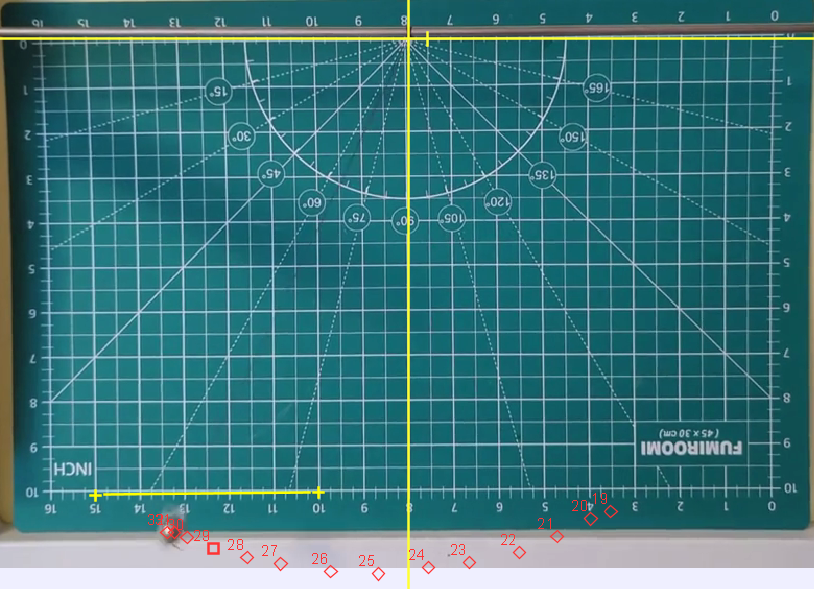
\includegraphics[width=0.75\linewidth]{pendulum.png}
	
	\newpage
	
	Опыт №1\\
	\(\theta_0 = 45^\circ\) градусов.\\
	Период \(T=1.10\).\\
	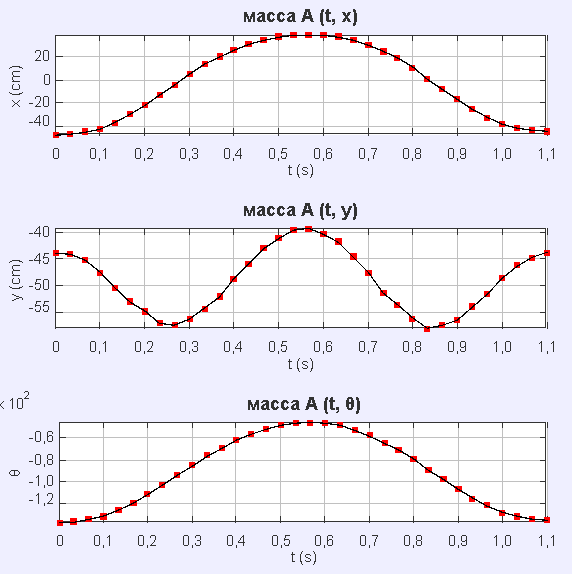
\includegraphics[width = 7cm, height = 7cm]{graph45.png}
	
	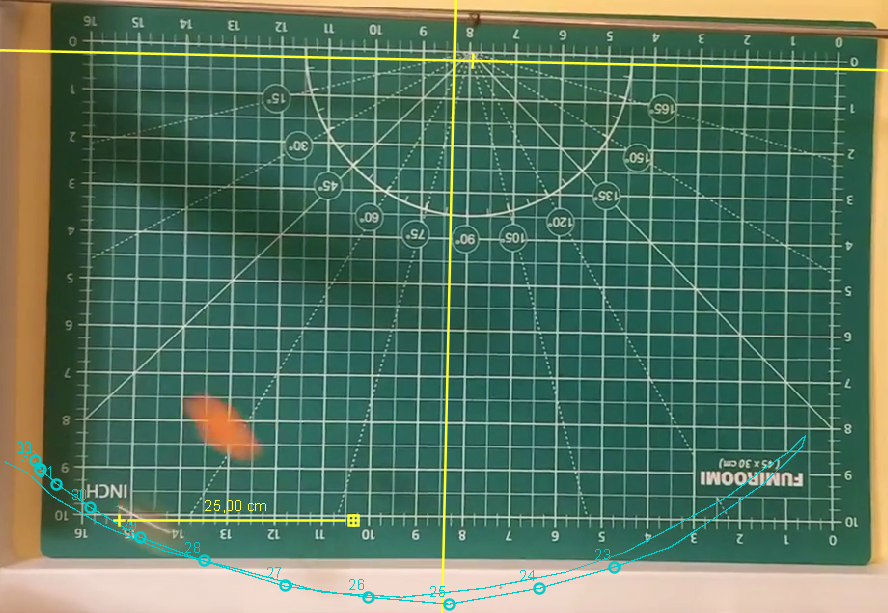
\includegraphics[width = 10cm, height = 8cm]{trajectory45.png}
	
	\newpage
	
	Опыт №2\\
	\(\theta_0 = 30^\circ\) градусов.\\
	Период \(T=1.03\)с.\\
	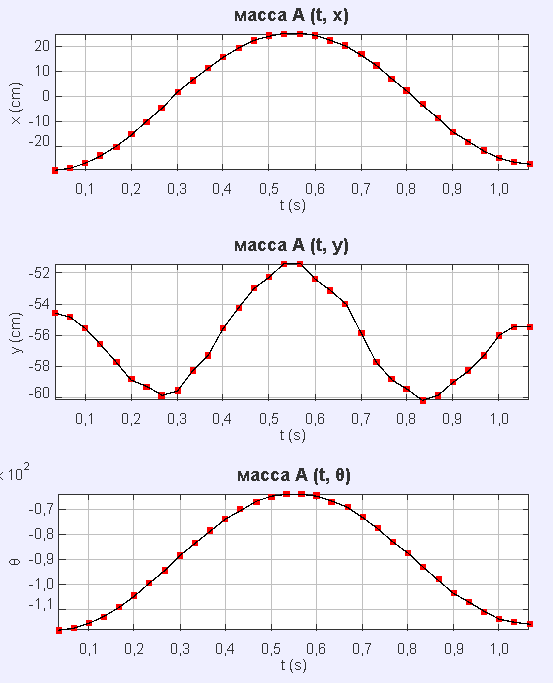
\includegraphics[width = 7cm, height = 7cm]{graph30.png}
	
	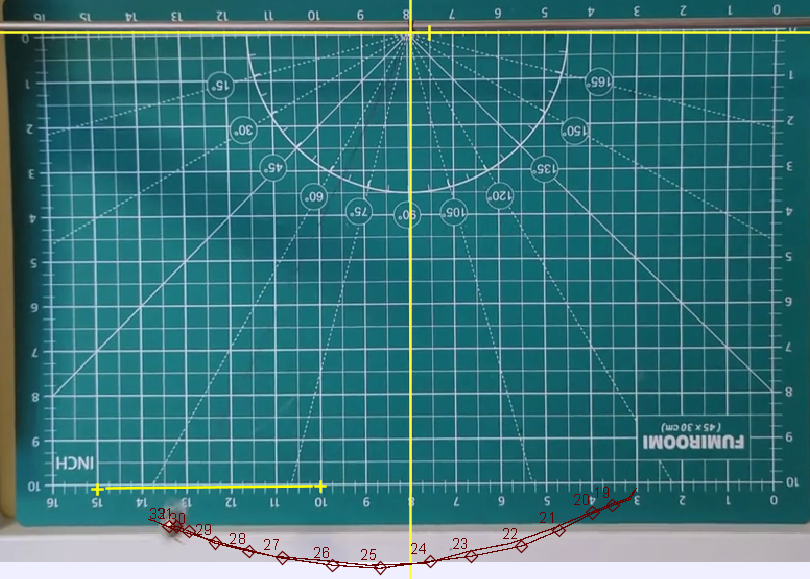
\includegraphics[width = 10cm, height = 8cm]{trajectory30.png}
	
	\newpage
	
	Опыт №3\\
	\(\theta_0 = 20^\circ\) градусов.\\
	Период \(T=1.00\)с.\\
	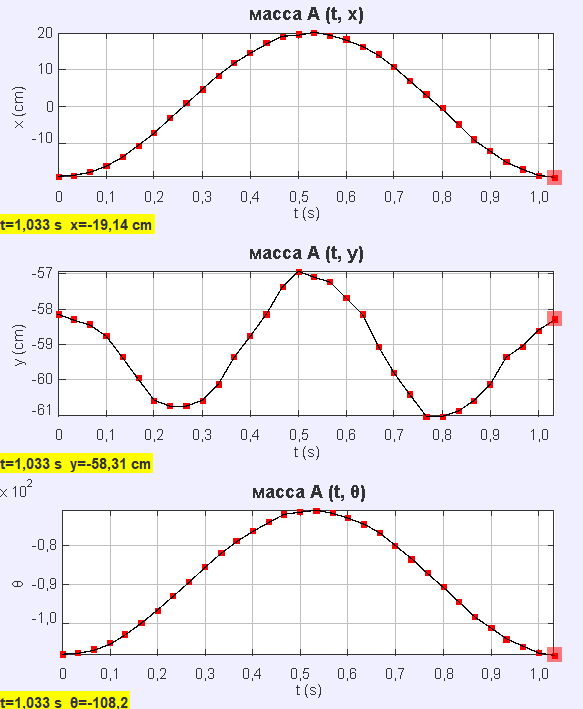
\includegraphics[width = 7cm, height = 7cm]{graph20.png}
	
	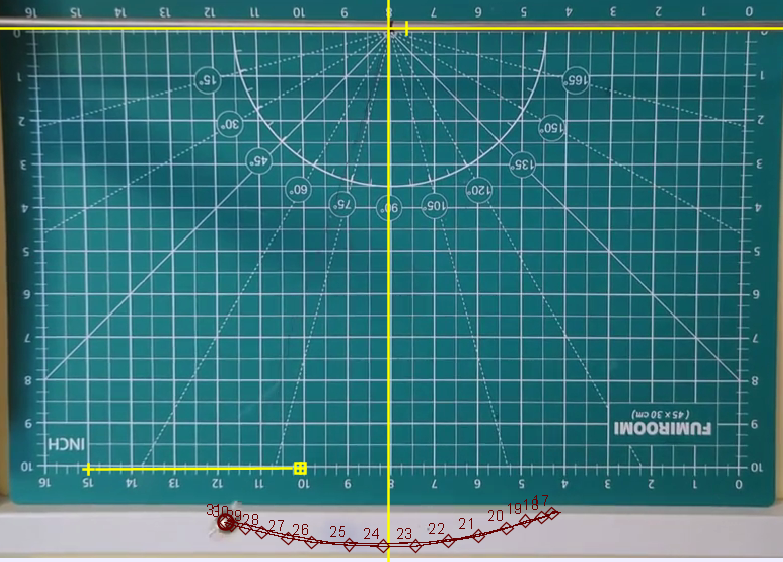
\includegraphics[width = 10cm, height = 8cm]{trajectory20.png}
	
	
	\newpage
	
	\large \textbf{\textcolor{structure.fg}{Отличие теории от практики}}\\
	
	формула (5)
	\[T=\frac{2\sqrt{2}}{\omega}\int\limits_0^{\theta_0}{\frac{d\theta}{\sqrt{\cos{\theta}-\cos{\theta_0}}}}.\]
	
	Главная загвоздка в комьютерном расчитывании этого интеграла в том, что выражение под корнем может равнятся нулю, то есть произойдет деление на 0. Чтобы такого не проиходило, мы как только можем уменьшим верхний предел и сделаем максимально мелкое разбиение.
	
	Реализация такой программы на языке python будет выглядеть примерно так:
	
	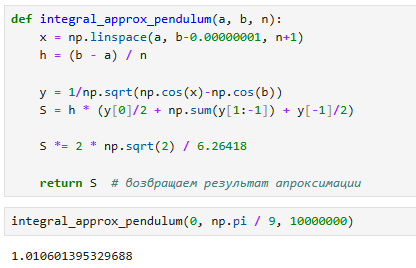
\includegraphics[width=10cm, height = 7cm]{pendulum_approx.png}
	\newpage

Опыт №1\\
\(T_{\text{прак}}=1.10\).\\
\(T_{\text{теор}}=\frac{2\sqrt{2}}{6.26418}\int\limits_0^{\pi/4}{\frac{d\theta}{\sqrt{\cos{\theta}-0.707106}}}=1.043573\)\\

Опыт №2\\
\(T_{\text{прак}}=1.03\).\\
\(T_{\text{теор}}=\frac{2\sqrt{2}}{6.26418}\int\limits_0^{\pi/6}{\frac{d\theta}{\sqrt{\cos{\theta}-0.866025}}}=1.020415\)\\

Опыт №3\\
\(T_{\text{прак}}=1.00\).\\
\(T_{\text{теор}}=\frac{2\sqrt{2}}{6.26418}\int\limits_0^{\pi/7.2}{\frac{d\theta}{\sqrt{\cos{\theta}-0.906307}}}=1.0150\)\\
	\newpage
	
	\large \textbf{\textcolor{structure.fg}{Доказательство (6)}}\\
	
	Требуется доказать, что
	\[\int\limits_0^{\theta_0}\frac{d\theta}{\sqrt{\cos{\theta}-\cos{\theta_0}}}=\sqrt{2}F\left(\frac{\pi}{2}, \sin{\frac{\theta_0}{2}}\right)\]
	
	Доказательство:
	
	1. Используем тригонометрическое тождество(\(\cos{x}=1-2\sin^2{\frac{\theta}{2}}\)).
	
	\[\cos{\theta}-\cos{\theta_0}=2\left(\sin^2{\frac{\theta_0}{2}}-\sin^2{\frac{\theta}{2}}\right)\]
	
	2. Подставляем интеграл.
	\[I=\int\limits_0^{\theta_0}\frac{d\theta}{\sqrt{2(\sin^2\frac{\theta_0}{2}-\sin^2\frac{\theta}{2})}}\]
	\newpage
	3. Замена переменной.\\
	Пусть \(\sin\frac{\theta}{2}=k\sin{\varphi}\), где \(k=\sin\frac{\theta_0}{2}\).\\
	При \(\theta=0: \sin{0}=k\sin\varphi\Rightarrow\varphi=0\).\\
	При \(\theta=\theta_0: \sin{\frac{\theta_0}{2}}=k\sin\varphi\Rightarrow\sin\varphi=1\Rightarrow\varphi=\frac{\pi}{2}\).\\
	
	Дифференцируем замену:\\
	\[\frac{1}{2}\cos\frac{\theta}{2}d\theta=k\cos\varphi\ d\varphi\]
	
	Выражаем \(d\theta\):\\
	\[d\theta=\frac{2k\cos\varphi}{\cos\frac{\theta}{2}}d\varphi\]
	
	\(\cos\frac{\theta}{2}=\sqrt{1-\sin^2\frac{\theta}{2}}=\sqrt{1-k^2\sin^2\varphi}\), следовательно:
	\[d\theta=\frac{2k\cos\varphi}{\sqrt{1-k^2\sin^2\varphi}}d\varphi\]
	\newpage
	
	4. Знаменатель исходного интеграла:
	\[\sqrt{2(k^2-k^2sin^2\varphi)}=\sqrt{2k^2(1-sin^2\varphi)}=\sqrt{2}k \cos\varphi\]
	
	5. Подставляем все в интеграл:
	\[I=\int\limits_0^{\pi/2}\frac{\frac{2k \cos\varphi}{\sqrt{1-k^2\sin^2\varphi}}d\varphi}{\sqrt{2}k \cos\varphi}=\sqrt{2}\int\limits_0^{\pi/2}\frac{d\varphi}{\sqrt{1-k^2sin^2\varphi}}\]
	
	Таким образом \[I=\sqrt{2}F\left(\frac{\pi}{2},\sin\frac{\theta_0}{2}\right)\]
	
	\newpage
	
	\large \textbf{\textcolor{structure.fg}{Эллиптический интеграл}}\\
	
	\[K(k)=\int\limits_0^{\pi/2}\frac{du}{\sqrt{1-k^2\sin^2{u}}}=
	\frac{\pi}{2}\sum\limits_{n=0}^{\infty}\left(\frac{(2n-1)!!}{(2n)!!}k^n\right)^2\]
	
	Для \(n=0\):\\
	\(\left(\frac{(2n-1)!!}{(2n)!!}k^n\right)^2=\left(\frac{(-1)!!}{(0)!!}\right)^2=1^2=1\)\\
	
	Для \(n=1\):\\
	\(\left(\frac{(2n-1)!!}{(2n)!!}k^n\right)^2=
	\left(\frac{(1)!!}{(2)!!}k\right)^2=\left(\frac{1}{2}k\right)^2=\frac{k^2}{4}\)\\
	
	Для \(n=2\):\\
	\(\left(\frac{(2n-1)!!}{(2n)!!}k^n\right)^2=
	\left(\frac{(3)!!}{(4)!!}k^2\right)^2=
	\left(\frac{1 \cdot 3}{2 \cdot 4}k^2\right)^2=\frac{9k^4}{64}\)\\
	
	Значит при \(n=2\):\\
	\[K(k)=\frac{\pi}{2}\left(1+\frac{k^2}{4}+\frac{9k^4}{64}\right)\]
	
	\newpage
	
	Полный эллиптический интеграл первого рода может использоваться для расчетов периода колебаний математического маятника с большой амплитудой. Например по вот такой формуле:
	
	\[T=\frac{4}{\omega _{0}}K\left(\sin \frac{\theta _{0}}{2}\right)\]
	\newpage
	Рассмотрим \(\theta_0 = 30^{\circ}, \sin{\frac{\theta_0}{2}=0.2588}\) для примера с нашим маятником. Тогда 
	
	\textcolor{orange}{При \(n=0\):}\\
	\(T=\frac{4}{6.26418}K\left(\sin \frac{\theta_{0}}{2}\right)=
	0.638551 \cdot \frac{\pi}{2}=1.00302\)\\[0.5cm]
	
	\textcolor{orange}{При \(n=1\):}\\
	\(T=\frac{4}{6.26418}K\left(\sin \frac{\theta_{0}}{2}\right)=
	0.638551 \cdot \frac{\pi}{2}(1+\frac{\sin^2{\frac{\theta_0}{2}}}{4})=
	1.00302 \cdot (1+\frac{0.2588^2}{4})=1.00302 \cdot 1.016746 = 1.0198165\)\\[0.5cm]
	
	\textcolor{orange}{При \(n=2\):}\\
	\(T=\frac{4}{6.26418}K\left(\sin \frac{\theta_{0}}{2}\right)=
	0.638551 \cdot \frac{\pi}{2}(1+\frac{\sin^2{(15^\circ)}}{4}+\frac{9\sin^4{(15^\circ)}}{64})=
	1.00302 \cdot (1+\frac{0.2588^2}{4}+\frac{0.2588^4}{64})=
	1.00302 \cdot (1 + 0.016746 + 0.000070) = 1.0198868\)\\
	
	\newpage
	
	\large \textbf{\textcolor{structure.fg}{Оценка погрешностей и выводы}}\\
	Во время проведения эксперимента источником погрешности были:
	\begin{itemize}
		\item Неточность измерения длины L.
		\item Неточность определения угла \(\theta_0\).
		\item Сопротивление воздуха, трение в подвесе.
		\item Малая частота кадров, плохое качество видео.
	\end{itemize}
	А во время вычислений:
	\begin{itemize}
		\item Погрешность компьютерных вычислений.
		\item Погрешность от использования конечного числа членов ряда (7).
	\end{itemize}
	\textbf{Выводы}:
	
	Нелинейная модель точнее описывает движение при больших амплитудах.
	
	Ряд (7) позволяет удобно вычислять период без численного интегрирования, но при больших углах требует многих членов.
	
\end{document}